%
% Tesi D.S.I. - modello preso da
% Stanford University PhD thesis style -- modifications to the report style
%
%%%%%%%%%%%%%%%%%%%%%%%%%%%%%%%%%%%%%%%%%%%%%%%%%%%%%%%%%%%%%%%%%%%%%%%%%%%
%                                                                         %
%			TESI DOTTORATO                                                %
%			______________                                                %
%                                                                         %
%			AUTORE: Andrei Ciulpan                                        %
%                                                                         %
%			Ultima revisione: 15.06.2019                                  %
%                                                                         %
%%%%%%%%%%%%%%%%%%%%%%%%%%%%%%%%%%%%%%%%%%%%%%%%%%%%%%%%%%%%%%%%%%%%%%%%%%%
%
%
\documentclass[12pt]{report}
%    \renewcommand{\baselinestretch}{1.6}      % interline spacing
%
% \includeonly{}
%
%			PREAMBOLO
%
\usepackage[a4paper]{geometry}
\usepackage{amssymb,amsmath,amsthm}
\usepackage{graphicx}
\usepackage[hyphens,spaces,obeyspaces]{url}
\usepackage{hyperref}
\usepackage{epsfig}
\usepackage[italian]{babel}
\usepackage{tesi}
\usepackage{afterpage}
\usepackage[font=small,labelfont=bf]{caption}
\usepackage{subcaption}
\usepackage{tabularx}
\usepackage{enumerate}
\usepackage{float}
\usepackage{wrapfig}
\usepackage{tikz}
\usepackage{xcolor}
\usepackage{listings}

\renewcommand{\UrlFont}{\footnotesize}

\newcolumntype{L}{>{\raggedright\arraybackslash}X}

\addto{\captionsitalian}{%
	\renewcommand{\bibname}{Sitografia}
}

\renewcommand{\lstlistingname}{Listato} % Listing -> Listato

\definecolor{mygreen}{rgb}{0,0.6,0}
\definecolor{mygray}{rgb}{0.5,0.5,0.5}
\definecolor{mymauve}{rgb}{0.58,0,0.82}

\definecolor{lightgray}{rgb}{.9,.9,.9}
\definecolor{darkgray}{rgb}{.4,.4,.4}
\definecolor{purple}{rgb}{0.65, 0.12, 0.82}


\lstdefinelanguage{Node}{
	keywords={do, if, in, for, let, new, try, var, case, else, eval, null, this, true, void, with, await, break, catch, class, const, false, super, throw, while, yield, delete, export, import, public, return, static, switch, typeof, extends, finally, package, private, continue, debugger, function, arguments, interface, protected, implements, instanceof
	},
	morecomment=[l]{//},
	morecomment=[s]{/*}{*/},
	morestring=[b]',
	morestring=[b]",
	ndkeywords=
	{
		class, 
		export, 
		boolean, 
		throw, 
		implements, 
		import, 
		this,
		console,
		\_\_dirname,
		locals,
		message,
		require,
		type, 
		required, 
		trim, 
		uppercase, 
		lowercase,
		enum,
		default,
		exports,
		\$eq,
		\_id,
	},
	keywordstyle=\color{cyan}\bfseries,
	ndkeywordstyle=\color{red}\bfseries,
	identifierstyle=\color{black},
	commentstyle=\color{mygreen}\ttfamily,
	stringstyle=\color{mymauve}\ttfamily,
	sensitive=true,
	captionpos=b
}

\lstdefinelanguage{JavaScript}{
	keywords={typeof, new, true, false, catch, function, return, null, catch, switch, var, const, let, async, await, if, in, while, do, else, case, break, from},
	ndkeywords={class, export, boolean, throw, implements, import, this},
	sensitive=false,
	comment=[l]{//},
	morecomment=[s]{/*}{*/},
	morestring=[b]',
	morestring=[b]",
	captionpos=b
}

\newcommand\blankpage{%
	\null
	\thispagestyle{empty}%
	\addtocounter{page}{-1}%
	\newpage}

% per le accentate
\usepackage[utf8]{inputenc}
%
\newtheorem{myteor}{Teorema}[section]
%
\newenvironment{teor}{\begin{myteor}\sl}{\end{myteor}}
%
%
%			TITOLO
%
\begin{document}
	

\title{Sistema Accessi IoT}
\author{Andrei CIULPAN}
\dept{Corso di Laurea in Informatica} 
\anno{2018/2019}
\matricola{872394}
\relatore{Andrea TRENTINI}
\correlatore{Marco LANZA}
\afterpage{\blankpage}
% 
%			DEDICA
%
\beforepreface

{\hfill \footnotesize {\sl Ringrazio i miei genitori e la nonna per il sostegno e per la pazienza che hanno avuto.}}
\vskip 0.8cm
{\hfill \footnotesize {\sl Ringrazio i miei amici e compagni di università per aver reso l'esperienza più bella e soprattutto più facile.}}
\vskip 0.8cm
{\hfill \footnotesize {\sl Ringrazio i miei tutor e colleghi per avermi dato la possibilità di crescere e concludere l'esperienza universitaria.}}

\afterpreface

%\listoffigures 

%\listoftables 

%			CAPITOLO 1: Intro
\chapter{Introduzione}\label{cap:introduzione}
%

Il controllo accessi è un sistema di protezione che permette l'accesso solo a determinate persone per via di qualche procedura di autenticazione: nel mondo fisico si può parlare di una semplice serratura (storicamente il sistema più utilizzato in assoluto) che può essere aperta solo dalle persone in possesso della chiave, mentre nel mondo dell'informatica si può notare l'enorme utilizzo delle procedure di autenticazione (login) che aiutano il sistema, tramite l'inserimento di un nome utente e password, a determinare automaticamente se una persona è autorizzata ad accedere alle risorse del sistema stesso.

Il controllo accessi\cite{controllo_accessi} è un tema molto sviluppato nel campo della sicurezza sia fisica che informatica: è stato segnalato che nel 2017, per il secondo anno consecutivo, il mercato del controllo accessi ha avuto la crescita più rapida nell'industria della sicurezza fisica\cite{crescita_controllo_accessi}. È inoltre un sistema onnipresente, utilizzato in ospedali, fabbriche, supermercati, aziende, sistemi di trasporto pubblico (e.g. l'ATM di Milano), case e tanti altri campi.  

La tesi si propone di trattare un sistema ibrido in cui il mondo fisico e il mondo informatico lavorano insieme: attraverso sensori ed attuatori è possibile avere la comunicazione tra i due mondi. 

Si tratta di un sistema \emph{Internet of Things} (IoT), ovvero un sistema in cui la connessione Internet viene estesa anche al mondo degli oggetti fisici (\emph{smart objects}\cite{smart_objects}) di uso comune. Gli oggetti si rendono riconoscibili e \textquotedblleft{} acquisiscono intelligenza \textquotedblright{} grazie al fatto di possedere una o più delle seguenti funzionalità: identificazione, localizzazione, diagnosi di stato, interazione con l'ambiente circostante, elaborazione dati e ovviamente connessione.
Gli oggetti intelligenti di un sistema IoT sono normalmente dotati di un processore embedded, sensori e attuatori e sono in grado di agire sui dati raccolti dall'ambiente e, ancora più importante, mandare questi dati in rete dove possono poi essere analizzati dal sistema centrale\cite{IoT}. Un semplice esempio di un sistema IoT si può trovare nella Figura \ref{fig:iot_diagram}.

\begin{figure}[H]
	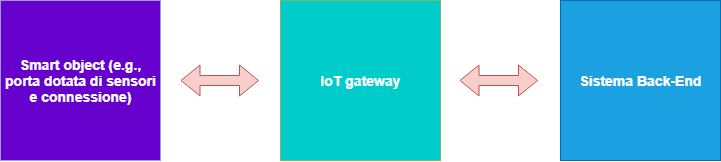
\includegraphics[width=\linewidth]{./img/iot_diagram.png}
	\caption{Esempio di sistema IoT}
	\label{fig:iot_diagram}
\end{figure}

Le seguenti sezioni di questo capitolo introdurranno il progetto stesso (denominato \emph{SimSim}) che poi verrà dettagliato nei prossimi capitoli.

%
\section{Nascita ed evoluzione del progetto all'interno dell'azienda}
%

SimSim è nato all'interno di \emph{Yatta}, il primo makerspace in centro a Milano. Yatta è uno spazio attrezzato con tecnologie e macchinari digitali destinato alla prototipazione e gestito da professionisti del settore 3D, programmazione, elettronica e grafica, in una visione ampliata del concetto di artigiano orientato verso la Manifattura e Industria 4.0. Gli studenti tirocinanti a Yatta sono inseriti nel laboratorio e partecipano allo sviluppo di progetti di physical computing che prevedono automazioni gestite tramite microcontrollori. Inizialmente SimSim aveva un unico scopo, ovvero quello di creare un sistema di accessi con la possibilità di salvare i log (su un cloud remoto o su una SD card) per poi leggerli. Quando ho iniziato a lavorare come tirocinante, esisteva già una versione iniziale del progetto (senza database e sito web) incompleta e, secondo me, abbastanza incasinata, perciò ho deciso di iniziare il tutto da capo. 

Durante la fase di sviluppo, l'idea del progetto è evoluta fino a diventare un sistema più completo, munito di un database per l'azienda e un sito web per gestirlo. Ho lavorato principalmente in autonomia ma sono stato aiutato anche dal tutor aziendale con alcune scelte progettuali come ad esempio la scelta di alcune componentistiche hardware, creazione degli schemi del database, scelta del template dell'interfaccia web, eccetera. Inoltre mi sono stati forniti tutti i materiali necessari alla creazione del prototipo, compresa la stampante 3D per la creazione della scatola (modello 3D nella Figura \ref{fig:simsim_3d}) e della porta progettate per il prototipo nella Figura \ref{fig:simsim}.

La sequenza temporale delle attività svolte si può vedere nella Figura \ref{fig:timeline}.

\pagebreak

\vspace*{80px}

\begin{figure}[H]
	\centering
	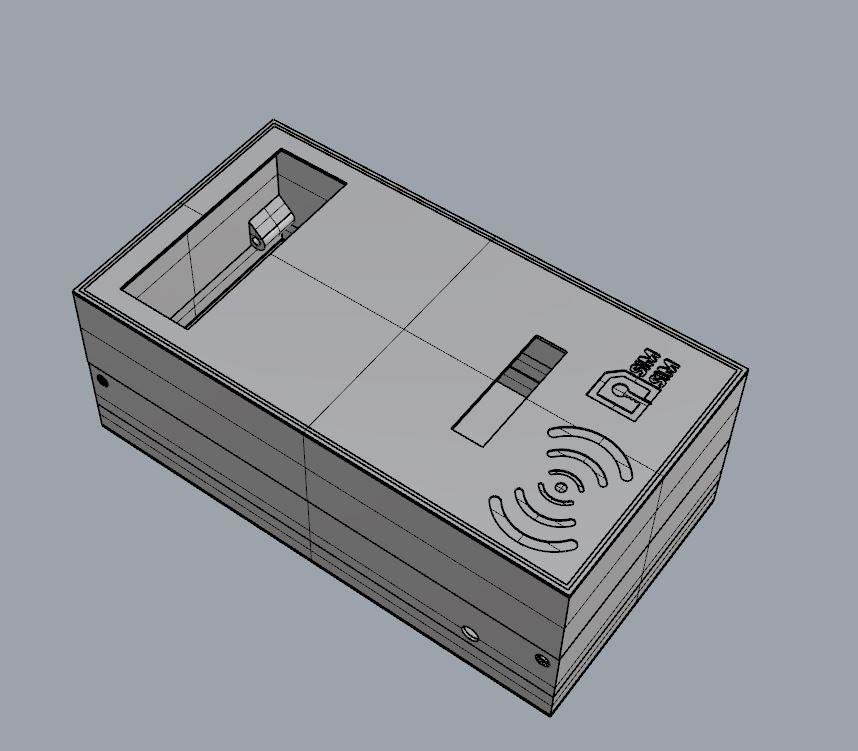
\includegraphics[width=0.9\linewidth]{./img/simsim_3d.jpeg}
	\caption{Modello 3D della scatola contenente il prototipo. Un ringraziamento alla mia collega Cecilia per la sua creazione}
	\label{fig:simsim_3d}
\end{figure}

\begin{figure}[H]
	\centering
	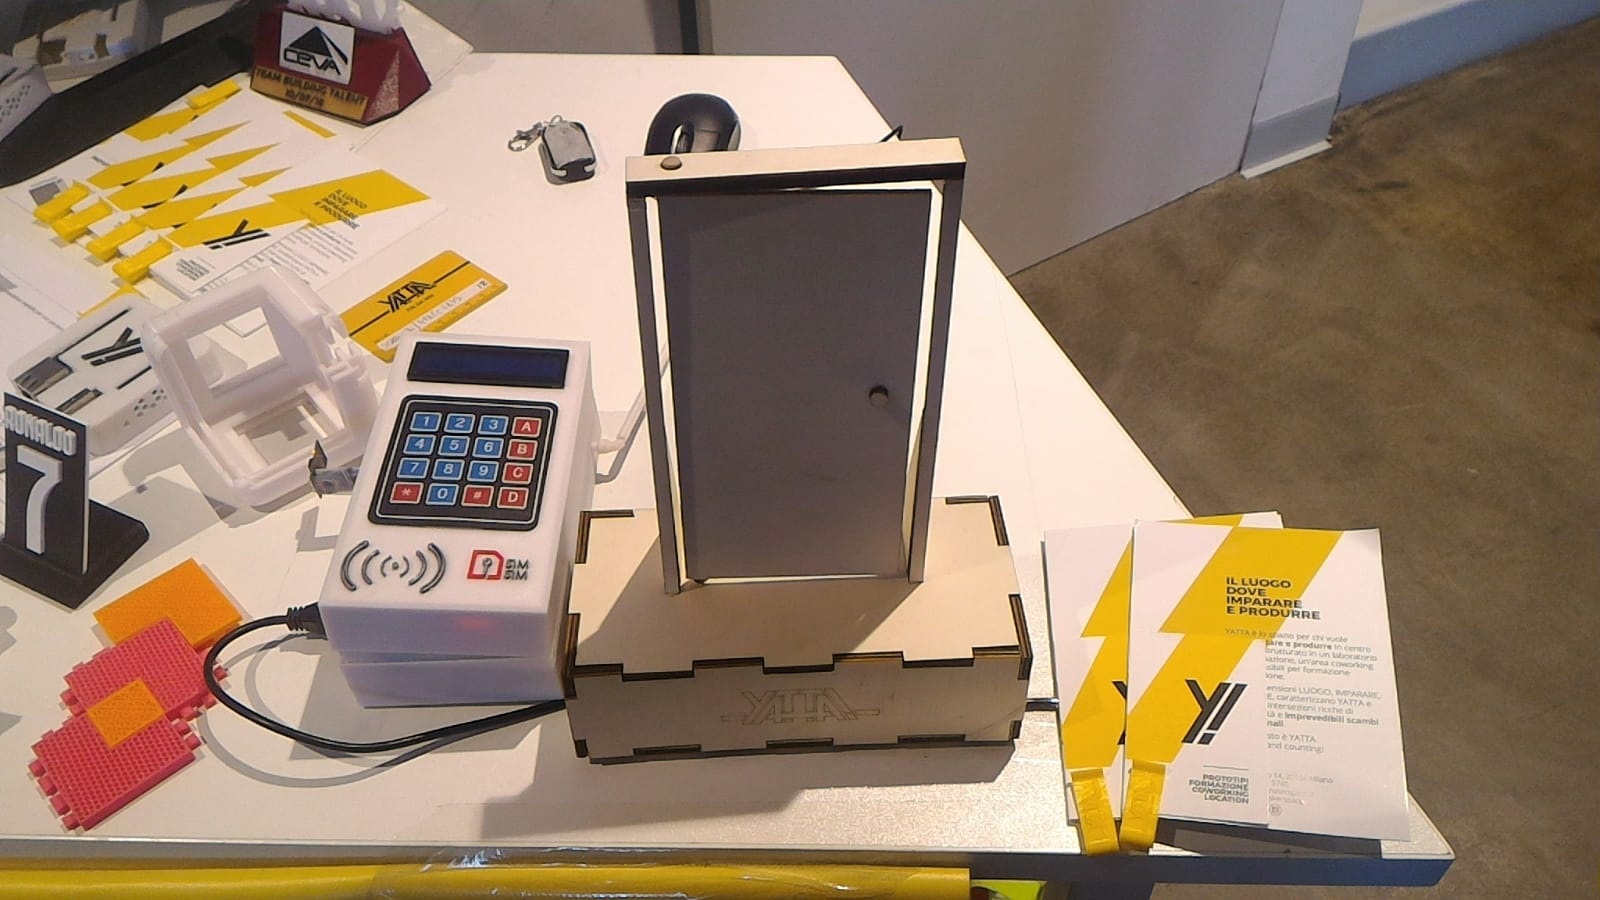
\includegraphics[width=0.8\linewidth]{./img/simsim.jpeg}
	\caption{Prototipo di SimSim}
	\label{fig:simsim}
\end{figure}

\pagebreak
  
%
\section{Requisiti del progetto}\label{sec:req}
%

L'attività principale del tirocinio è la realizzazione di un sistema di controllo accessi, da applicare presso varchi. Vengono elencati i requisiti del sistema:

\begin{enumerate}
	\item Deve essere in grado di funzionare con diverse modalità di riconoscimento:
	\begin{enumerate}
		\item Tessera RFID
		\item Tastierino numerico (password)
		\item Telecomando 
	\end{enumerate}
	\item Deve dare la possibilità di visualizzare su un display LCD ciò che sta succedendo (accesso consentito, accesso negato, inserimento password ecc.). Inoltre deve essere implementata una funzione che permette all'amministratore di visualizzare i codici delle tessere RFID sul display LCD (operazione protetta da una password).
	\item A seguito di ogni accesso avvenuto con successo deve aprire la serratura di una porta e salvare il log in un database remoto (in LAN o in un cloud) tramite WiFi.
	\item Deve avere un database per:
	\begin{enumerate}
		\item Tessere RFID
		\item Log degli accessi
		\item Soci
	\end{enumerate}
	\item Deve avere un'interfaccia grafica (in questo caso un sito web) tramite la quale l'utente amministratore possa gestire il database con le seguenti funzioni: 
	\begin{enumerate}
		\item Visualizzare/aggiungere/modificare/cancellare i soci 
		\item Visualizzare/aggiungere/modificare/cancellare le tessere 
		\item Visualizzare i log degli accessi
	\end{enumerate}
\end{enumerate}
I dispositivi scelti per soddisfare i requisiti sono stati un Arduino UNO (per la parte hardware) e un Raspberry Pi 3B+ su cui ospitare il server di database. 

Nelle Figure \ref{fig:usecase} e \ref{fig:flowchart} si possono trovare rispettivamente un diagramma dei casi d'uso e un diagramma di flusso del sistema.

\begin{figure}[H]
	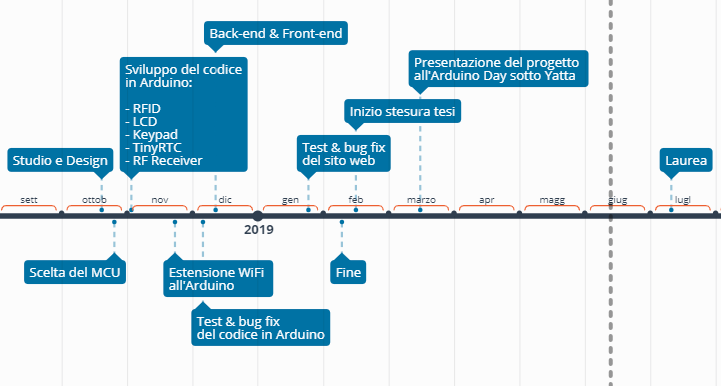
\includegraphics[width=\linewidth]{./img/timeline.png}
	\caption{Sequenza temporale delle attività svolte. Creato con il tool \url{https://time.graphics/it/editor}}
	\label{fig:timeline}
\end{figure}

\begin{figure}[H]
	\center{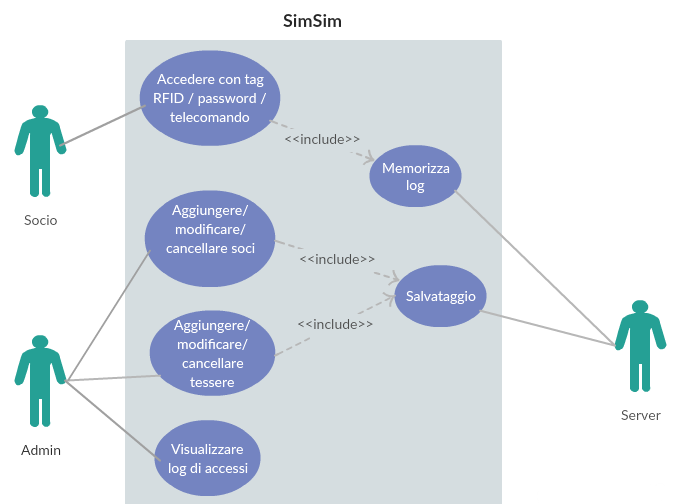
\includegraphics[width=0.8\linewidth]{./img/usecase.png}}
	\caption{Casi d'uso del sistema}
	\label{fig:usecase}
\end{figure}

\vspace*{75px} 

\begin{figure}[H]
	\center{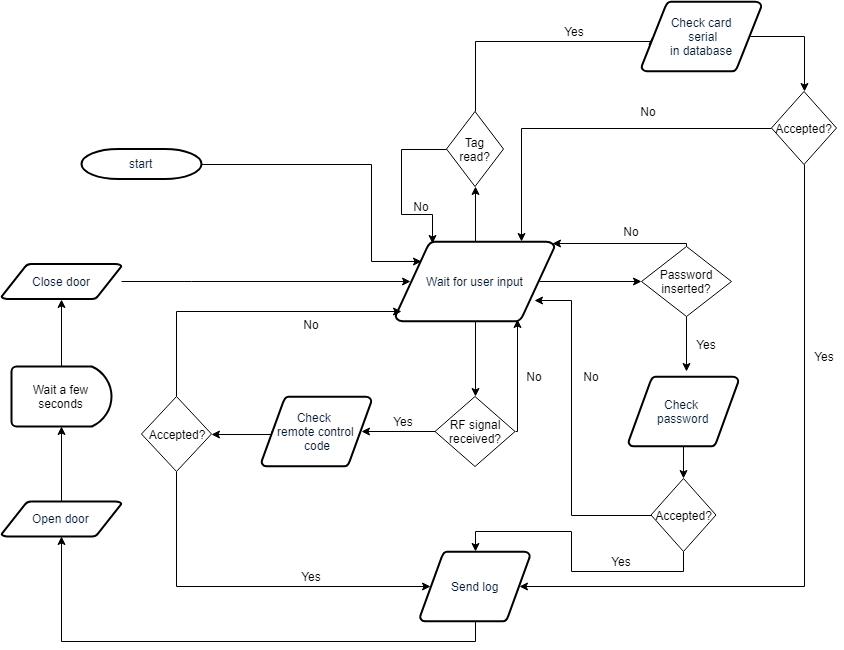
\includegraphics[width=1\linewidth]{./img/flowchart.png}}
	\caption{Diagramma di flusso del sistema}
	\label{fig:flowchart}
\end{figure}


%			CAPITOLO 2
\chapter{Sviluppo del sistema embedded}
\label{cap2}
%

\lstset{
	language=C++,
	basicstyle=\ttfamily\footnotesize\color{darkgray},
	keywordstyle=\color{cyan}\ttfamily,
	stringstyle=\color{mymauve}\ttfamily,
	commentstyle=\color{mygreen}\ttfamily,
	morecomment=[l][\color{magenta}]{\#},
	tabsize=2,
	numbers=left,                  
	numbersep=5pt,                   
	numberstyle=\tiny\color{mygray},
	breaklines=true,
	backgroundcolor=\color{white},
	showstringspaces=false,
	frame=single,
	extendedchars=true,
	morekeywords=
	{
		boolean,
		RCSwitch,
		Servo,
		Serial,
		LiquidCrystal\_PCF8574,
		Wire,
		byte,
		WiFi,
		String,
		HTTPClient,
		SoftwareSerial,
		JSON
	},
	captionpos=b
}

In questo capitolo vengono dettagliati i dispositivi hardware utilizzati all'interno del sistema embedded. Uno schema completo del circuito elettrico si trova nella Figura \ref{fig:schematics}.

\begin{figure}
	\center{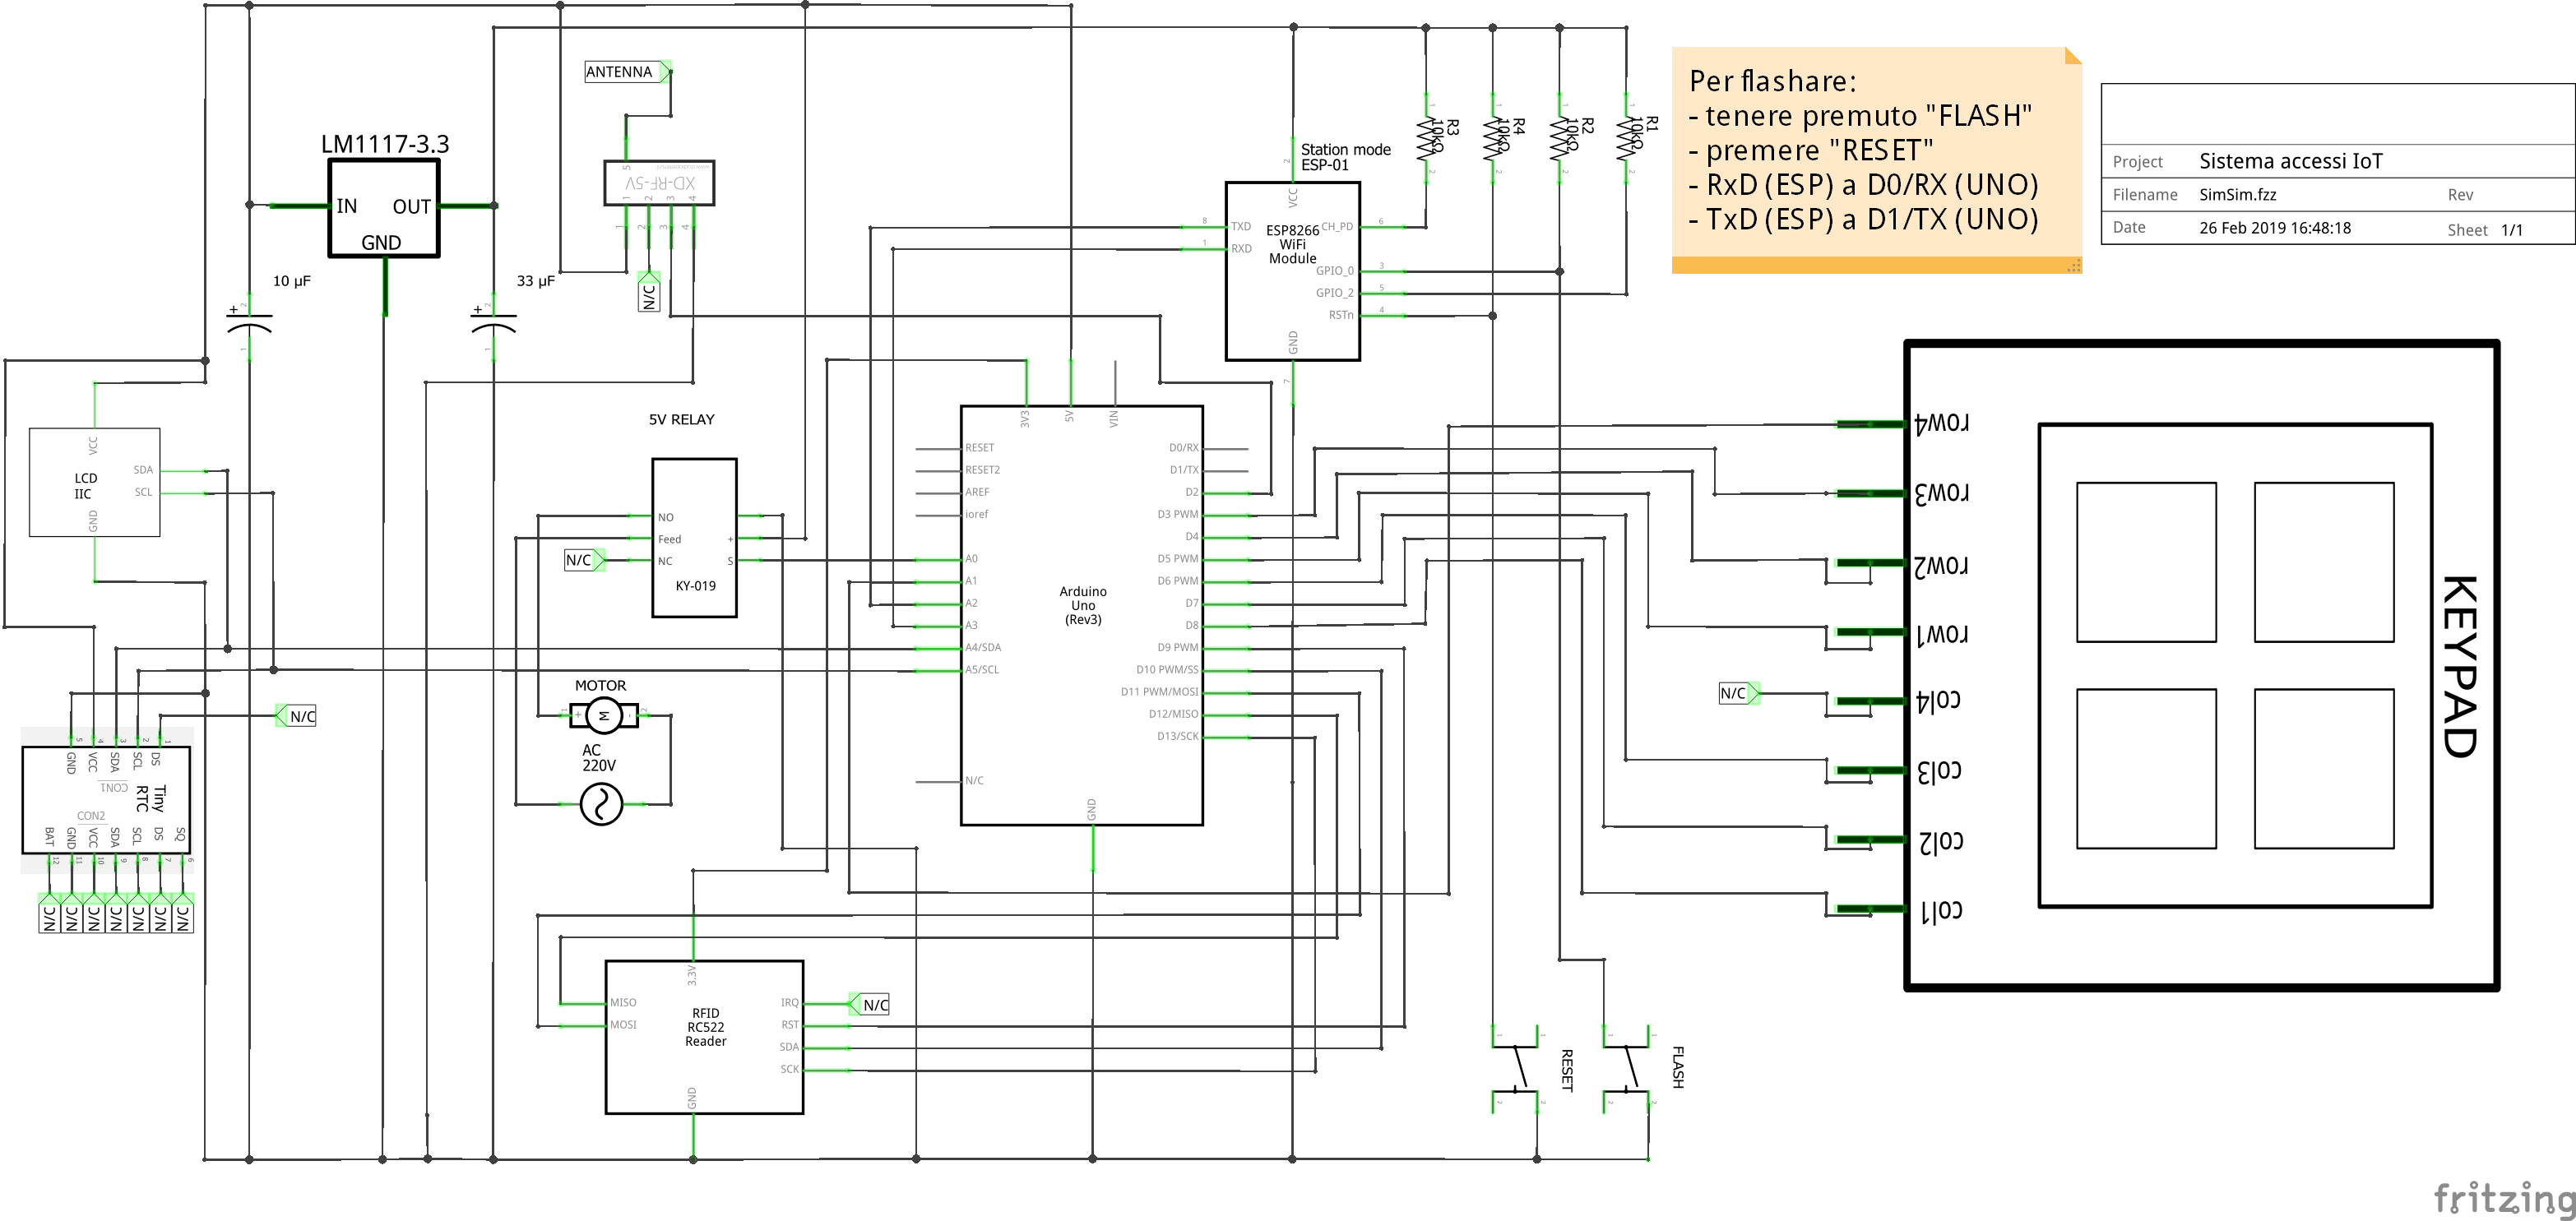
\includegraphics[width=\textwidth,height=1.1\textheight,keepaspectratio]{./img/schematics.png}}
	\caption{Schema del circuito}
	\label{fig:schematics}
\end{figure}


%
\section{Raspberry Pi}
%

\begin{figure}[H]
	\center{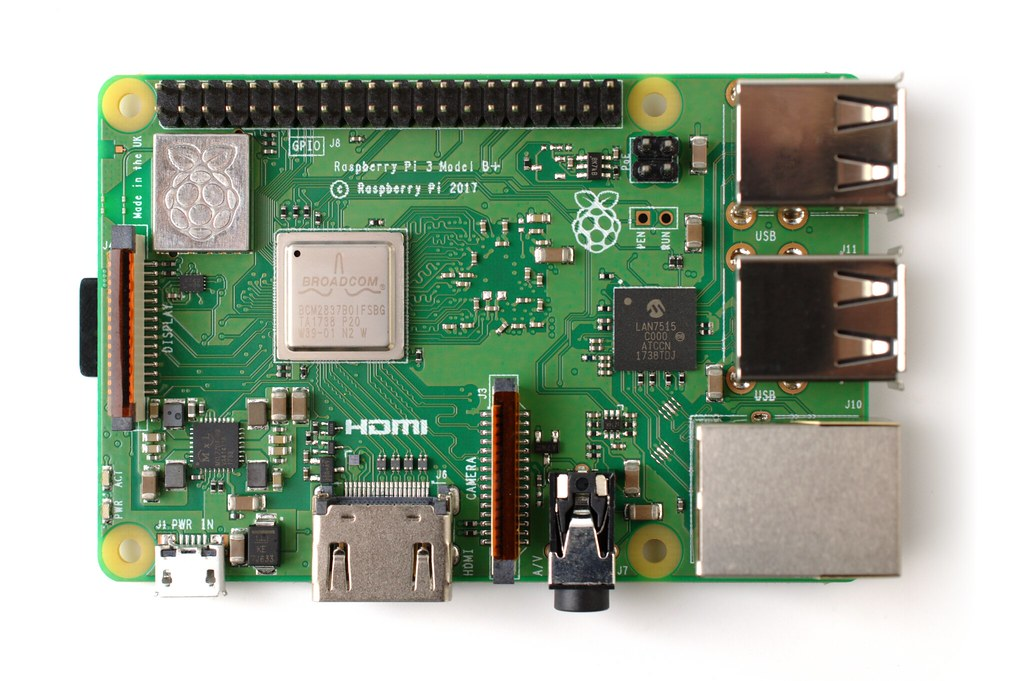
\includegraphics[width=0.35\linewidth]{./img/raspi.jpg}}
	\caption{Scheda Raspberry Pi}
	\label{fig:raspi}
\end{figure}

Raspberry Pi (Figura \ref{fig:raspi}) è una serie di piccoli computer (system-on-chip) dalle dimensioni simili a quelle di una carta di credito. La scheda è stata sviluppata nel Regno Unito (Fondazione Raspberry Pi). Le prime versioni avevano poca potenza computazionale e sono state progettate con l'intenzione di offrire a insegnanti e studenti uno strumento semplice e poco costoso con cui poter insegnare e imparare a programmare. La scheda ha avuto un enorme successo anche in altri campi (e.g$.$ robotica) e con ogni nuova versione è stata migliorata. Le ultime versioni sono assai potenti e possono essere utilizzate per tante altre cose. Le schede sono basate su sistemi operativi di tipo GNU/Linux, in particolare Raspbian che può essere scaricato dal sito della fondazione (\cite{raspbian}). 

La scheda utilizzata nel progetto (Raspberry Pi 3B+) possiede un'architettura su 64 bit, essenziale per poter utilizzare in maniera efficiente MongoDB (che è limitato a una memoria di 2 GB su un sistema a 32bit). 
Il Raspberry Pi 3B+ possiede inoltre una scheda WiFi, il che la rende un buon candidato per lo scopo principale del progetto, ovvero quello di ospitare il server.


%
\section{Arduino UNO}
%

Arduino\cite{arduino_storia} è nata ad Ivrea nel 2005 come piattaforma di prototipazione elettronica di basso costo e open-source (dettaglio molto importante che ha portato al successo che ha avuto) che si basa su hardware e software flessibili e facili da usare. Il nome della scheda deriva di quello del bar di Ivrea frequentato dai fondatori del progetto ed la scheda è stata creata per artisti, designer e hobbisti. Essendo open-source, ha avuto un grande successo nel mondo degli hobbisti, anche a livello mondiale (tale da diventare una delle invenzioni più considerevoli nella storia dell'elettronica), grazie alla facilità di programmazione, basso costo e soprattutto disponibilità in rete delle informazioni necessarie per poter permettere a persone con grandi idee e poche capacità informatiche ed elettroniche di realizzare i propri progetti. 

Al giorno d'oggi Arduino potrebbe anche non essere la scelta immediata, anzi, ormai ci sono schede più potenti, più veloci e con migliori rapporti prestazioni/prezzo, ma non scordiamoci che è tutto grazie agli sviluppatori della scheda. Perchè scegliere, quindi, un Arduino? Essendo la scheda che ha fatto partire tutto, è anche la scheda più studiata e ciò significa che gira intorno a più informazioni, più librerie già pronte, più dispositivi compatibili e ha anche un sito di appassionati che si aiutano a vicenda dove si possono trovare tutorial, libri e tant'altro.

La scheda utilizzata nel progetto, Arduino UNO (Figura \ref{fig:uno}), è assolutamente la scheda più conosciuta al mondo e si può ormai trovare a dei prezzi molto bassi (ci sono tanti clone diversi in rete grazie al fatto di essere OpenHardware). Tra le varie caratteristiche vengono elencate le più interessanti:

\begin{itemize}
	\item Microcontrollore: ATmega328 (datasheet: \url{https://www.sparkfun.com/datasheets/Components/SMD/ATMega328.pdf})
	\item Digital I/O Pins: 14 tra cui 6 offrono la funzione PWM (si veda la sezione \ref{sec:servomotore} \textquotedblleft{} Servomotore \textquotedblright{}) e 4 implementano il protocollo SPI (si veda la sezione \ref{sec:spi} \textquotedblleft{} SPI \textquotedblright{})
	\item Analog I/O Pins: 6 tra cui 2 implementano il protocollo I$^2$C (si veda la sezione \ref{sec:i2c} \textquotedblleft{} I$^2$C \textquotedblright{})
	\item Flash Memory: 32 KB
	\item EEPROM: 1 KB
	\item Clock Speed: 16 MHz
	\item DC Current per i pin I/O: max 40 mA
	\item DC Current per il pin 3V3: max 50 mA
	\item Operating Voltage: 5V
	\item Input Voltage (recommended): 7-12V
\end{itemize}

L'Arduino UNO è quindi un dispositivo ideale per il progetto; l'unica cosa che manca è la possibilità di accedere al WiFi, indispensabile per l'IoT, ma questo problema è stato risolto grazie ad un chip chiamato ESP8266 (si veda la sezione \ref{sec:esp8266} \textquotedblleft{} ESP8266 \textquotedblright{}).

\begin{figure}[H]
	\center{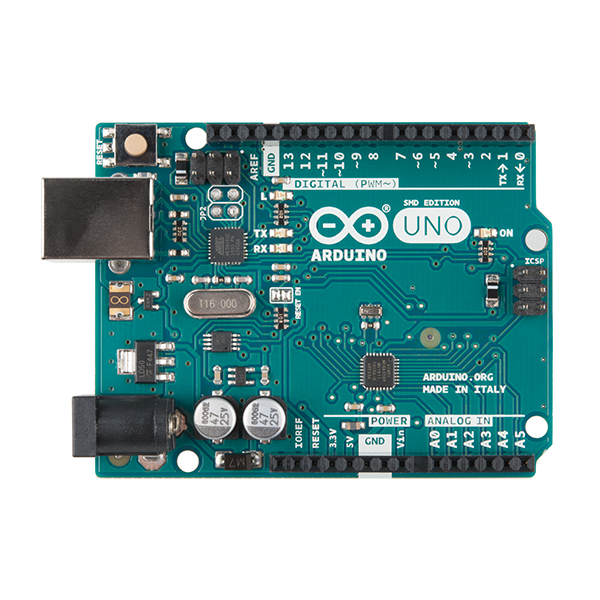
\includegraphics[width=0.35\linewidth]{./img/uno.jpg}}
	\caption{Scheda Arduino UNO}
	\label{fig:uno}
\end{figure}

%
\subsection{Arduino Programming Language}
%

La scheda Arduino UNO (e qualsiasi altra board compatibile con Arduino) può essere facilmente programmata utilizzando, ma non solo, l'\emph{Arduino IDE} (Arduino Integrated Development Software), un software sviluppato da Arduino.cc e funzionante sulle 3 piattaforme dominanti (Windows, Linux e MacOS). Il linguaggio di programmazione si chiama \textquotedblleft{} Arduino Programming Language \textquotedblright{}\cite{sistemi_embedded_atrent} ed è un derivato di Wiring, una piattaforma di sviluppo open-source composta da un linguaggio di programmazione, un IDE e un circuito stampato basato su un microcontrollore. La sintassi è molto simile a quella del linguaggio C/C++; infatti il linguaggio di programmazione di Arduino è un insieme di funzioni e librerie C/C++ che possono essere chiamate dal codice. Forse la cosa diversa e che si nota di più rispetto ad altri linguaggi di programmazione è la diversa strutturazione dello \emph{sketch} (sinonimo di programma): per poter funzionare vengono sempre definite due funzioni iniziali, \emph{setup()} e \emph{loop()}. La prima viene eseguita soltanto una volta all'avvio del programma e serve per dichiarare variabili, modalità dei pin (e.g. input o output) ecc., mentre nella seconda viene messo il programma vero e proprio che viene eseguito ripetutamente... all'infinito.


%
\section{Real-time Clock}
%

I requisiti del progetto richiedono il salvataggio del log dopo ogni accesso avvenuto con successo, e per fare ciò è necessario essere in grado di tenere traccia del tempo. Il Raspberry Pi, diversamente dai PC a cui siamo abituati, può tenere traccia del tempo solo se ha accesso alla connessione Internet per accedere ad un server NTP (Network Time Protocol); nel progetto in questione, il Raspberry Pi, nonostante sia connesso alla rete LAN, è stato privato della connessione Internet per questioni di sicurezza (nessun utente esterno alla rete può accedere al server in locale perciò elimina gran parte degli attacchi possibili). Ciò significa che, per poter avere il cosiddetto timestamp nei log, bisogna trovare un modo di tenere traccia della data e dell'ora. Fortunatamente esistono dei piccoli chip chiamati RTC che fanno questo lavoro. 

Nella Figura \ref{fig:tinyRTC} si può vedere il dispositivo utilizzato nel progetto, chiamato TinyRTC, un modulo basato sul clock chip DS1307 (datasheet: \url{https://datasheets.maximintegrated.com/en/ds/DS1307.pdf}) che supporta il protocollo I$^2$C (si veda la sezione \ref{sec:i2c} \textquotedblleft{} I$^2$C \textquotedblright{}) per cui è facilmente utilizzabile dall'Arduino UNO.
L'orologio può essere programmato con la data e l'ora corrente direttamente con il programma dell'Arduino e, grazie alla batteria al litio (CR1225), continua a tenere traccia del tempo anche senza alimentazione esterna. Il dispositivo è in grado di fornire, con abbastanza precisione, data e ora in termini di secondi, minuti, ora, giorno, mese e anno. Grazie alla popolarità di Arduino ci sono tante librerie per che permettono il facile utilizzo del dispositivo; nel progetto è stata usata una libreria chiamata RTClib (\cite{RTClib}). Nella Figura \ref{fig:tinyRTC_uno} si può vedere il collegamento con l'UNO.

\begin{figure}[H]
	\centering
	\begin{minipage}{0.5\textwidth}
		\centering
		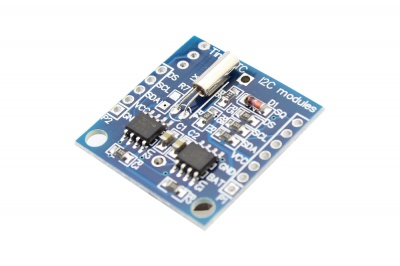
\includegraphics[width=0.5\linewidth]{./img/tinyRTC.jpg}
		\captionof{figure}{Tiny RTC}
		\label{fig:tinyRTC}
	\end{minipage}%
	\begin{minipage}{0.5\textwidth}
		\centering
		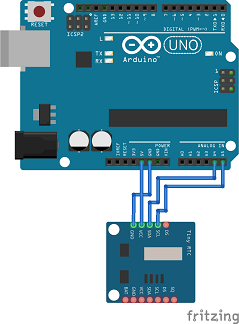
\includegraphics[width=0.55\linewidth]{./img/tinyRTC_uno.png}
		\captionof{figure}{Tiny RTC e Arduino UNO}
		\label{fig:tinyRTC_uno}
	\end{minipage}
\end{figure}

%
\section{Trasmettitore-ricevitore RF}
%

\begin{figure}[H]
	\center{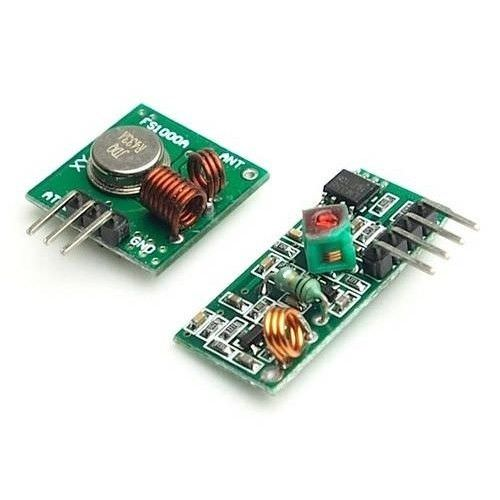
\includegraphics[width=0.25\linewidth]{./img/receiver_transmitter_module.jpg}}
	\caption{Modulo transceiver MX-05V/XD-RF-5V}
	\label{fig:rx_tx_module}
\end{figure}

Ci sono due principali tipi di tecnologie per i telecomandi: a raggi infrarossi o a radio-frequenza (RF).
La tecnologia a raggi infrarossi è quella più utilizzata ed è usata da tanti dispositivi elettronici (un esempio molto comune è il telecomando della TV). In questo caso trasmettitore e ricevitore devono essere messi faccia a faccia e non troppo distanti tra di loro, perciò non è il caso di usare questa tecnologia nel progetto (non si potrebbe, ad esempio, aprire la porta stando dietro ad un muro).

La tecnologia scelta è quindi quella a radio-frequenza, in cui trasmettitore e ricevitore possono comunicare anche se sono messi in camere diverse. Il dispositivo scelto (Figura \ref{fig:rx_tx_module}) è un modulo composto da trasmettitore e ricevitore in radio-frequenza a 433 MHz (\cite{rf}). Il trasmettitore è stato utilizzato soltanto per programmare i telecomandi dell'azienda con i codici voluti grazie alla loro funzione di clonazione (codice nel Listato \ref{lst:trasm}).

\begin{lstlisting}[caption={L'Arduino utilizza il trasmettitore per trasmettere i codici clonati dai telecomandi. Il codice viene inviato per 4 volte ogni 3 secondi}, label={lst:trasm}]
#include <RCSwitch.h>

int i = 0;
const char code[24] = "011100011011000110011010";
RCSwitch mySwitch = RCSwitch();

void setup() {
	Serial.begin(9600);
	mySwitch.enableTransmit(A0);
	mySwitch.setPulseLength(600);
	mySwitch.setProtocol(1);
}

void loop() {
	i = 0;
		while (i < 4) {
		mySwitch.send(code);
		i++;
		delay(400);
	}
	delay(3000);
}
\end{lstlisting}

Il ricevitore, invece, è sempre collegato all'Arduino (Figura \ref{fig:rf_uno}) e riesce a ricevere i segnali mandati dai telecomandi anche da qualche decina di metri di distanza. Se il codice che viene mandato dal telecomando è corretto allora l'Arduino lo risconosce e apre la porta, altrimenti fa finta di niente. 

\begin{figure}[H]
	\center{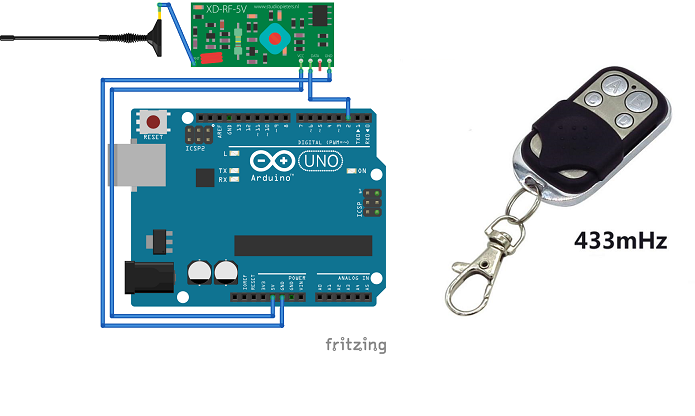
\includegraphics[width=0.6\linewidth]{./img/rf_uno.png}}
	\caption{Ricevitore RF con telecomando e Arduino UNO}
	\label{fig:rf_uno}
\end{figure}

Il ricevitore, per aumentare il range, è stato accoppiato con un'antenna lunga 17,3 cm. Il motivo di questa scelta è che la lunghezza dell'antenna deve essere 1/4 di quella della lunghezza d'onda. Bisogna quindi calcolare la lunghezza d'onda $\lambda$:
%
\[\lambda(m) = \frac{v(m/s)}{f(Hz)} = \frac{299,792,458}{433,000,000} = 0,692 m\] 
%
dove \textit{v} è la velocità della luce e \textit{f} è la frequenza (433 MHz). Ora si può trovare la lunghezza \emph{L} dell'antenna: 
%
\[L = \frac{\lambda}{4} = \frac{0,692}{4} = 0,173m = 17,3 cm \]
%

%
\section{Servomotore}\label{sec:servomotore}
%

\begin{figure}[H]
	\center{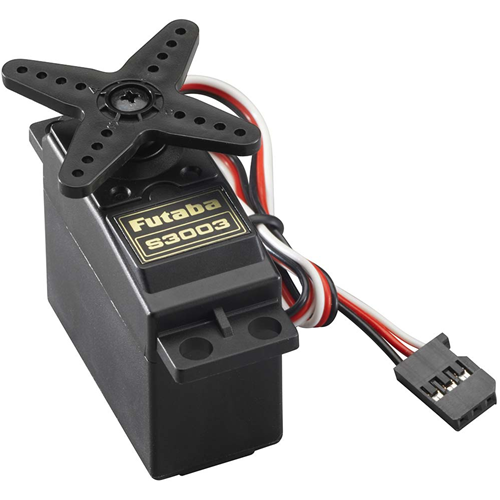
\includegraphics[width=0.15\linewidth]{./img/servo.png}}
	\caption{Servomotore}
	\label{fig:servo}
\end{figure}
Esistono tanti tipi diversi di motori Arduino-compatibili, ognuno con i propri punti forti e deboli, perciò bisogna valutare bene quale scegliere in base alle necessità del progetto. In questo caso il lavoro del motore è semplice: deve girare la serratura di una porta da una parte e dall'altra, quindi senza particolare precisione, velocità o potenza. Siccome non c'è nemmeno il bisogno di avere una rotazione completa (bastano 180$^{\circ}$), è immediato pensare al servomotore che è anche facilmente controllabile da un Arduino grazie ai suoi pin PWM.

Il servomotore (Figura \ref{fig:servo}) è un dispositivo elettromeccanico a basso consumo energetico ed è costituito da un motore DC, un gruppo di ingranaggi (per ridurre le rotazioni al minuto e aumentare il momento torcente), un circuito di controllo (un ponte-H integrato), un potenziometro interno e un contenitore di plastica che lo racchiude. La particolarità del servomotore è che può ruotare con una precisione di alcuni gradi (normalmente da 0$^{\circ}$ a 180$^{\circ}$) in base alla larghezza dell'impulso che riceve. Questa è una tecnica che si chiama PWM.

Il motore è collegato al potenziometro attraverso gli ingranaggi: quando esso ruota, la resistenza del potenziometro cambia e quindi il circuito di controllo può misurare esattamente in quale direzione punta l'albero del motore. Quando l'albero del motore è arrivato alla posizione desiderata, esso si ferma perchè il circuito di controllo toglie l'alimentazione. Questo succede perchè vengono comparati due segnali: quello in ingresso e quello del potenziometro (che dipende dalla posizione dell'albero del motore). La differenza tra i due segnali produce un segnale chiamato \emph{segnale d'errore} che viene usato come input (dopo essere stato amplificato) al motore per farlo girare. Questo errore può essere sia positivo che negativo facendolo quindi girare sia da una direzione che dall'altra. Siccome il motore continua a girare, il segnale del potenziometro cambia, fino a essere uguale a quello in ingresso: quando si arriva a questo punto il segnale d'errore è pari a zero e ciò significa che non c'è più alimentazione e il motore si ferma. Come si può notare, il servomotore funziona sulla base della retroazione.

%
\subsection{PWM}
%

\emph{Pulse Width Modulation} (PWM) è una tecnica che consiste in un treno di impulsi di larghezza variabile che determinano la posizione del servo. È quindi un modo di ricavare un risultato analogico a partire da un segnale digitale. 

\begin{wrapfigure}{r}{0.5\textwidth}
	\begin{center}
		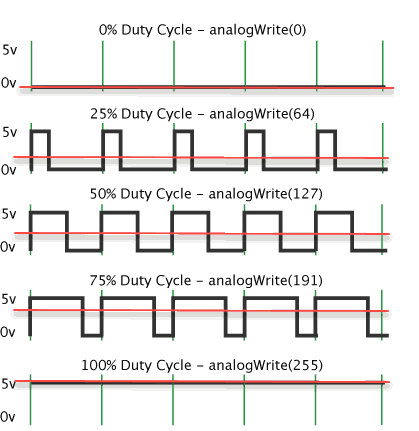
\includegraphics[width=0.9\linewidth]{./img/pwm.png}
		\captionof{figure}{Segnali PWM e comando analogWrite(int value) per generarli con l'Arduino. La \textit{Veff} è rappresentata dalla linea orizzontale rossa che copre il segnale digitale}
		\label{fig:pwm}
	\end{center}
\end{wrapfigure}

Un segnale PWM ha una forma d'onda quadra, con periodo fisso, ma spesso non simmetrica: la durata della semi-onda alta può variare (si veda la Figura \ref{fig:pwm}). La durata \textit{T[ON]} del segnale alto viene misurata in percentuale e si chiama \emph{duty cycle}: ad esempio un duty cycle del 25\% significa che \textit{T[ON]} dura per 1/4 della durata del periodo fisso \textit{T}. Questo tipo di segnale non è un vero e proprio segnale analogico, però può essere interpretato come tale: quello che succede è che la tensione viene applicata e levata nel giro di alcuni frazioni di secondo perciò quello che si chiama tensione efficace è in realtà minore della tensione reale applicata. Per calcolare la tensione efficace \textit{Veff} basta sapere la tensione applicata \textit{Vcc} e il duty cycle \textit{DC} (che si trova facendo il rapporto tra \textit{T[ON]} e \textit{T}):

%
\[Veff = Vcc \cdot DC\]
%
Generalmente, nel caso dei servomotori, si ha un periodo totale \textit{T} = 20 ms, perciò ogni 20 ms il servo riceve un nuovo impulso. La posizione del motore dipende quindi dalla durata del tempo \textit{T[ON]} che questo impulso rimane ad un livello logico HIGH. Nel grafico della Figura \ref{fig:servo_pwm} si può vedere che la durata dell'impulso alto è un valore compreso tra 1ms (duty dycle = 5\%) e 2ms (duty cycle = 10\%). Fissata la posizione centrale del servo a 90$^{\circ}$, allora abbiamo che: 


\begin{itemize}
	\item se la durata del livello logico HIGH dell'impulso sta nell'intervallo [1ms, 1.5ms] allora il servo ruota verso sinistra a partire dalla posizione centrale (la sua posizione varia tra 0$^{\circ}$ e 90$^{\circ}$);
	\item se la durata del livello logico HIGH dell'impulso è uguale a 1.5ms allora il servo resta fermo a 90$^{\circ}$;
	\item se la durata del livello logico HIGH dell'impulso sta nell'intervallo [1.5ms, 2ms] allora il servo ruota verso destra a partire dalla posizione centrale (la sua posizione varia tra 90$^{\circ}$ e 180$^{\circ}$).
\end{itemize}

\begin{figure}[H]
	\center{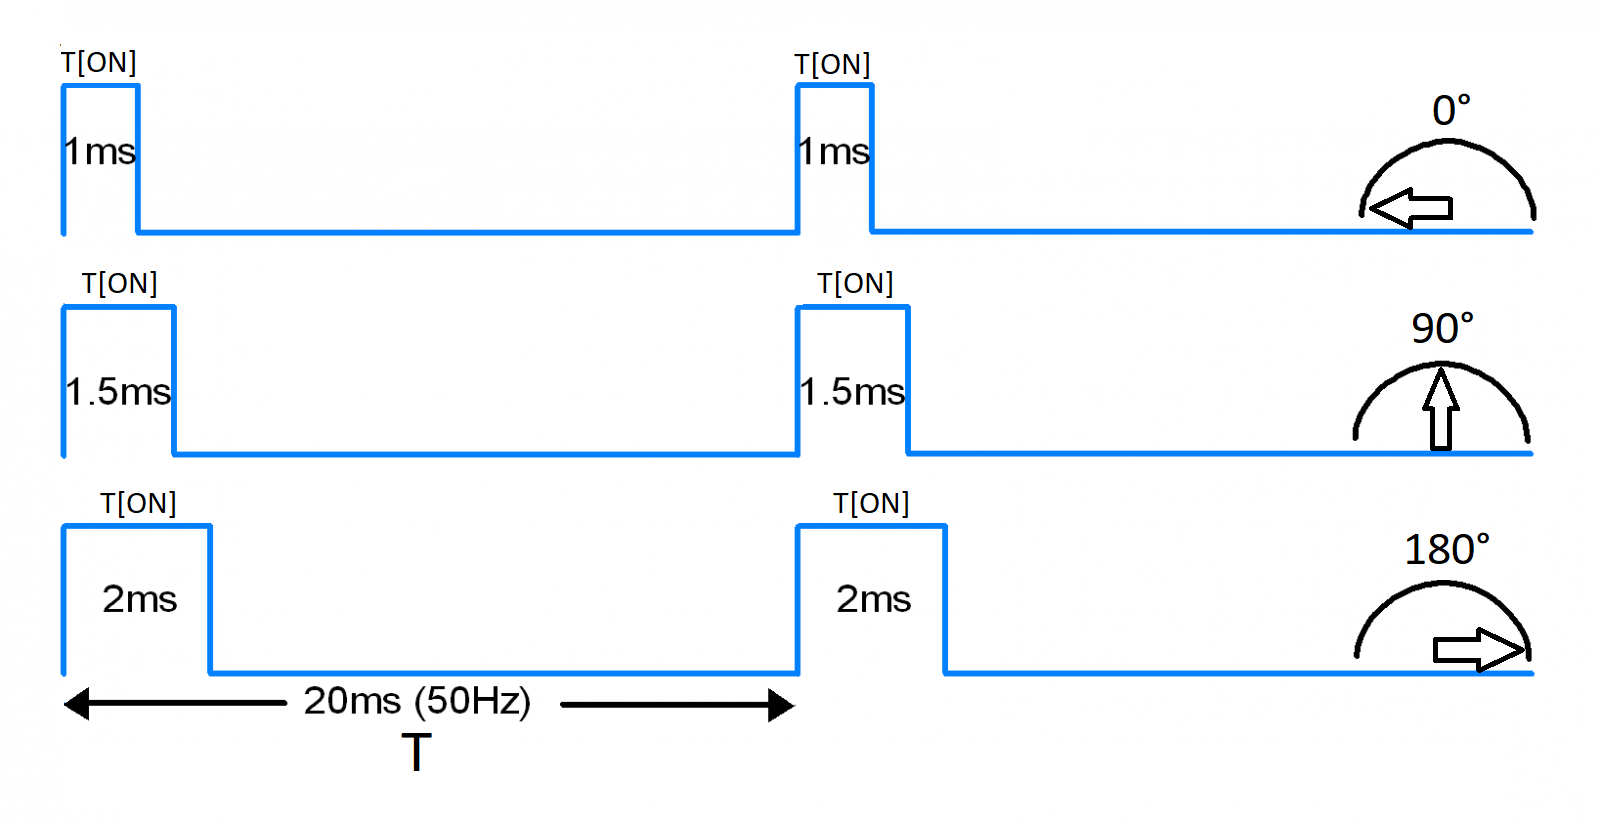
\includegraphics[width=0.9\linewidth]{./img/servo_pwm.png}}
	\caption{Segnali PWM nel servomotore}
	\label{fig:servo_pwm}
\end{figure}

Controllare un servomotore con l'Arduino è in realtà semplice perché esiste una libreria chiamata Servo (\cite{servo}) che ne facilita il lavoro: basta pensare in gradi. Nella Figura \ref{fig:servo_uno} viene fatto vedere un esempio di collegamento tra il servo e l'Arduino e un esempio di codice per controllarlo si trova nel Listato \ref{lst:servo}.

\begin{figure}[H]
	\center{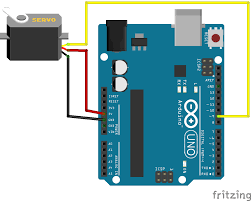
\includegraphics[width=0.3\linewidth]{./img/servo_uno.png}}
	\caption{Servomotore e Arduino UNO}
	\label{fig:servo_uno}
\end{figure}

\begin{lstlisting}[caption={Esempio di codice per controllare il servomotore: innanzittutto il servo viene collegato al pin 9 dell'Arduino e viene fatto ruotare di 180 gradi da una parte (aprendo la porta); dopo 5 secondi viene fatto ruotare di 180 gradi dalla parte opposta}, label={lst:servo}]
#include <Servo.h>

Servo myservo;
int pos = 0;

void setup() {
	myservo.attach(9);
}

void open() {
	for (pos = 0; pos <= 180; pos += 1) {  
		myservo.write(pos);				 
		delay(15);                      
	}
	delay(5000);
	for (pos = 180; pos >= 0; pos -= 1) {  
		myservo.write(pos);				   
		delay(15);                        
	}
}
\end{lstlisting}

%
\section{RFID Reader}
%

\emph{Radio Frequency Identification} (RFID) è un termine utilizzato per descrivere tecnologie contactless che fanno uso delle onde radio per identificare oggetti, persone e animali sia da vicino (tag passivi) che da lontano (tag attivi). L'identificazione è resa possibile grazie ad un lettore RFID in grado di interrogare i cosidetti tag, ovvero dei dispositivi elettronici di varie forme e dimensioni che possiedono i dati necessari per l'identificazione e che principalmente si dividono in due categorie: 

\begin{itemize}
	\item i tag passivi che sono poco costosi e contengono un'antenna e un piccolo chip con identificativo univoco e privo di alimentazione. Questi tag vengono utilizzati per l'identificazione a breve distanza (pochi centimetri) e vengono \textquotedblleft{} attivati \textquotedblright{} dalle onde radio del lettore;
	\item i tag attivi che sono più costosi e permettono, grazie all'alimentazione interna (emettono loro stessi i segnali radio), l'identificazione a lunga distanza (fino a 200 metri).
\end{itemize}

La tecnologia RFID si diversifica anche nella frequenza e trova utilizzo in tanti campi diversi quali gestione accessi, tracciabilità degli animali, gestione dei biglietti elettronici, ecc$.$ (per le basse e medie frequenze), ma anche in Telepass, identificazione di auto in movimento, tracciabilità degli oggetti in movimento ecc. (per le frequenze alte e altissime).

\begin{figure}
	\center{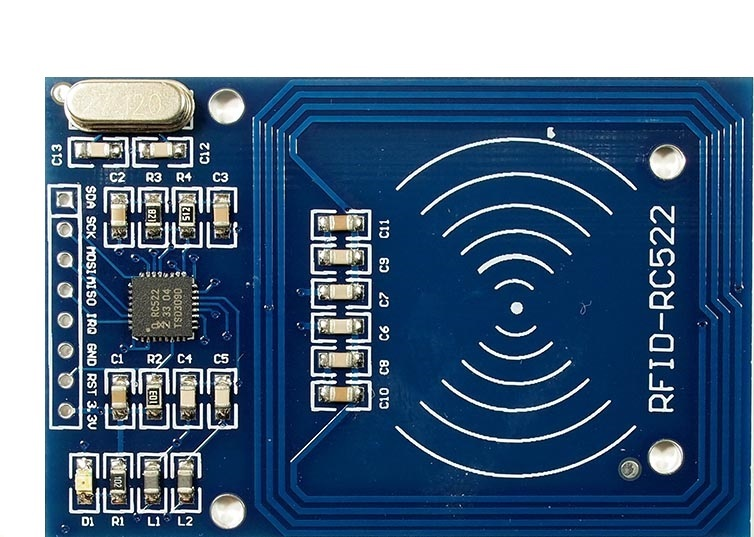
\includegraphics[width=0.23\linewidth]{./img/mfrc522.jpg}}
	\caption{Lettore RFID MFRC522}
	\label{fig:mfrc522}
\end{figure}

Il lettore RFID utilizzato nel progetto è chiamato MFRC522 (datasheet: \url{https://www.nxp.com/docs/en/data-sheet/MFRC522.pdf}) ed è illustrato nella Figura \ref{fig:mfrc522}. Esso opera su una frequenza di 13.56 MHz ed è in grado di comunicare con i tag che si conformano allo standard ISO/IEC 14443 A/MIFARE. Implementa vari protocolli di comunicazione (SPI, Serial UART, I$^2$C) ma è stata sviluppata solo una libreria per Arduino (\cite{rfid_lib}) basata sul protocollo SPI (si veda la sezione \ref{sec:spi} \textquotedblleft{} SPI \textquotedblright{}).

Nella Figura \ref{fig:rfid_uno} si trova il circuito per collegare il lettore RFID con l'UNO e un esempio di codice di Arduino per leggere i tag si trova nel Listato \ref{lst:rfid}.

\begin{figure}[H]
	\center{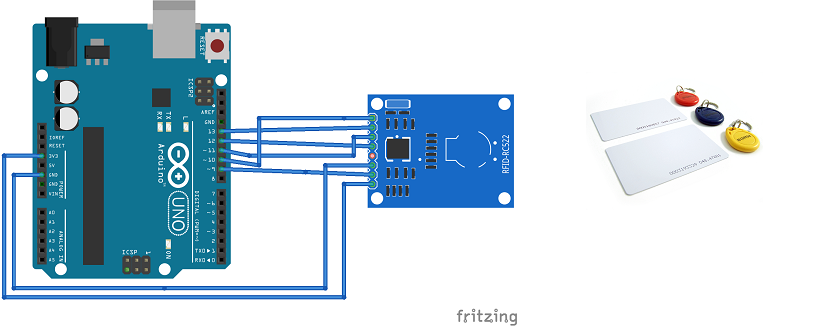
\includegraphics[width=0.7\linewidth]{./img/rfid_uno.png}}
	\caption{RFID con dei tag e Arduino UNO}
	\label{fig:rfid_uno}
\end{figure}

\begin{lstlisting}[caption={Procedura per leggere i tag. Essi vengono letti un byte alla volta e poi vengono concatenati in una stringa accessibile dal resto del programma}, label={lst:rfid}]
boolean rfidCardRead(void) {
	if ( !rfid.PICC_IsNewCardPresent() ) return false;
	if ( !rfid.PICC_ReadCardSerial() ) return false;
	currentCardNumber = "";
	for ( uint8_t i=0; i<5; i++ ) {
		currentCardNumber.concat(String(rfid.uid.uidByte[i], HEX));
	}
	currentCardNumber.toUpperCase();
	rfid.PICC_HaltA(); 
	return true;
}
\end{lstlisting} 

%
\section{Display LCD 16x2}
%
\begin{figure}[H]
	\center{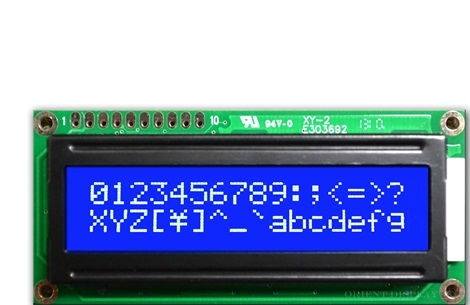
\includegraphics[width=0.35\linewidth]{./img/16x2.jpg}}
	\caption{Display LCD 16x2}
	\label{fig:16x2}
\end{figure}

I moduli LCD trovano ampio utilizzo nei sistemi embedded grazie al basso costo, disponibilità e utilità. Il display utilizzato si chiama \textquotedblleft{} 16x2 LCD \textquotedblright{} (Figura \ref{fig:16x2}) proprio perchè possiede uno schermo su cui si possono scrivere 2 linee di 16 caratteri ciascuna. Questi dispositivi sono abbastanza complessi (ci sono 1280 pixel da indirizzare) e per poterli utilizzare in maniera semplice ed efficiente è necessario avere un'interfaccia. Infatti i display LCD spesso vengono accoppiati con un controller che rende la vita facile al programmatore. Il controller più utilizzato (è considerato uno standard \textit{de facto}) si chiama HD44780 (datasheet: \url{https://www.sparkfun.com/datasheets/LCD/HD44780.pdf}), costruito dalla Hitachi, ed è in grado di controllare display LCD capaci di visualizzare solo caratteri. L'HD44780 supporta il trasferimento parallelo a 8 bit (possiede 8 bit di dati) e il suo compito principale è di ricevere i comandi e i dati in arrivo dall'MCU per poi processarli
e mandarli all'LCD.

Il problema principale dell'LCD 16x2, come si può vedere nella Tabella \ref{tab:lcd_pinout}, è il numero di pin necessari da collegare (e la pazienza per farlo) all'Arduino per poter farlo funzionare correttamente. Questo significa che, siccome l'Arduino ha un numero limitato di pin (13 digitali e 6 analogici), essi potrebbero non bastare per un progetto di dimensioni più grandi. Fortunatamente c'è una soluzione: I$^2$C (si veda la sezione \ref{sec:i2c} \textquotedblleft{} I$^2$C \textquotedblright{}). Esiste un chip che rende possibile la riduzione del numero di pin utilizzati a due, SDA e SCL, cambiando l'interfaccia parallela del controller in una seriale. Questo chip si chiama PCF8574 I/O Expander ed è definito come un backpack (è letteralmente uno zaino che si salda sopra l'LCD) e permette appunto all'LCD e all'Arduino di comunicare utilizzando il protocollo I$^2$C. In Arduino si può utilizzare una libreria già esistente chiamata LiquidCrystal\_PCF8574 (\cite{lcd_lib}) che sfrutta la libreria Wire (\cite{wire}) per implementare alcune funzioni utili al programmatore. Esempio di codice nel Listato \ref{lst:lcd}:
\begin{lstlisting}[caption={L'Arduino inizializza la comunicazione con l'LCD tramite il protocollo I$^2$C e chiama la funzione lcdHomeMode() che semplicemente spegne la retroilluminazione e pulisce il testo.}, label={lst:lcd}]
LiquidCrystal_PCF8574 lcd(lcdAddr); // lcdAddr = 0x27

void lcdSetup(void) {
	Wire.beginTransmission(lcdAddr);
	if ( Wire.endTransmission() == 0 ) Serial.println(F("LCD OK"));
	else Serial.println(F("LCD MISSING"));
	lcd.begin(16,2);
	lcd.noBlink();
	lcdHomeMode();
}

void lcdHomeMode(void) {
	lcd.setBacklight(0);
	lcd.clear();
}

\end{lstlisting}

\begin{table}[H]
	\begin{center}
		\begin{tabular}{l|l} 
			\textbf{Pin} & \textbf{Funzione del pin} \\
			\hline
			1 & Vss (GND) \\
			2 & Vcc (5V) \\ 
			3 & Vee (Contrasto) \\
			4 & RS (Register Select: 0 per selezionare l'invio di un comando, 1 per i dati) \\
			5 & R/W (Read/Write: 0 per la scrittura di dati/comandi, 1 per la lettura dati/stato) \\
			6 & E (Enable bit: inizia il ciclo di scrittura o lettura) \\
			7 & D0 (Data 0) \\
			8 & D1 (Data 1) \\
			9 & D2 (Data 2) \\
			10 & D3 (Data 3) \\
			11 & D4 (Data 4) \\
			12 & D5 (Data 5) \\
			13 & D6 (Data 6) \\
			14 & D7 (Data 7) \\
			15 & A (Anodo (+): retroilluminazione) \\
			16 & K (Catodo (-): retroilluminazione) \\
		\end{tabular}
	\caption{Pinout di un display LCD 16x2 con il controller HD44780}
	\label{tab:lcd_pinout}
	\end{center}
\end{table}

%
\section{Keypad}
%

\begin{figure}[H]
	\centering
	\begin{subfigure}{.5\textwidth}
		\centering
		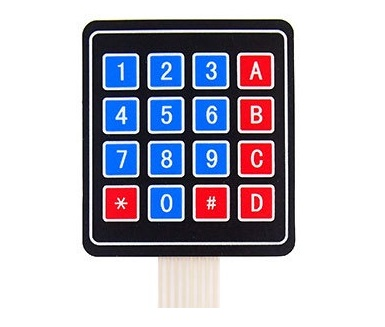
\includegraphics[width=0.6\linewidth]{./img/keypad.jpg}
		\caption{}
		\label{fig:keypad}
	\end{subfigure}%
	\begin{subfigure}{.5\textwidth}
		\centering
		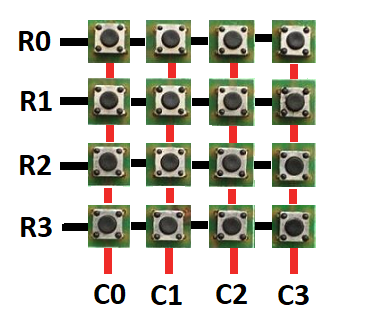
\includegraphics[width=0.58\linewidth]{./img/keypad_matrix.png}
		\caption{}
		\label{fig:keypad_matrix}
	\end{subfigure}
	\caption{\textbf{(a)} Tastierino 4x4 e \textbf{(b)} la sua rappresentazione a matrice}
	\label{fig:keypad_both}
\end{figure}

I tastierini sono dei dispositivi di input ampiamente utilizzati per dare la possibilità alle persone di interagire con un sistema (e.g$.$ inserire una password, controllare un robot ecc.). Normalmente i tasti sono disposti in un formato a matrice (in questo caso 4x4, ovvero 16 pulsanti) e permettono ad un microcontrollore di capire facilmente quale tasto è stato premuto in base alle linee che si attivano: nella Figura \ref{fig:keypad_both} si può facilmente vedere che premendo il pulsante \textquotedblleft{} 2 \textquotedblright{} vengono attivate le linee \textquotedblleft{} R0 \textquotedblright{} e \textquotedblleft{} C1 \textquotedblright{} e il microcontrollore, grazie a come è stato configurato, è in grado di dire che quel pulsante specifico è stato premuto. Un esempio di configurazione in Arduino del tastierino si può trovare nel Listato \ref{lst:keypad}. 
\begin{lstlisting}[caption={Configurazione dei pin del tastierino. In questo caso non viene utilizzata l'ultima colonna con le lettere.}, label={lst:keypad}]
const byte keypadRows = 4;   // quattro righe
const byte keypadCols = 3;  // tre colonne
const byte keypadRowPins[keypadRows] = {5, 4, 3, 15}; // 15 = A1
const byte keypadColPins[keypadCols] = {8, 7, 6};
const char keypadConfig[keypadRows][keypadCols] =
{
{'1','2','3'},
{'4','5','6'},
{'7','8','9'},
{'*','0','#'}
};
\end{lstlisting}

Le funzioni per utilizzare il tastierino sono implementate nella libreria Keypad di Arduino (\cite{keypad_lib}). Nella Figura \ref{fig:keypad_uno} si può vedere un esempio di collegamento tra il tastierino e l'Arduino UNO.


\begin{figure}[H]
	\center{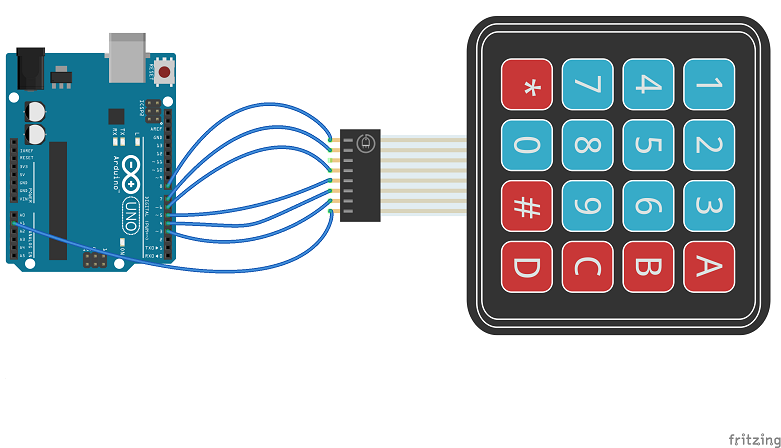
\includegraphics[width=0.6\linewidth]{./img/keypad_uno.png}}
	\caption{Keypad e Arduino UNO}
	\label{fig:keypad_uno}
\end{figure}


%
\section{ESP8266}\label{sec:esp8266}
%

\begin{figure}[H]
	\center{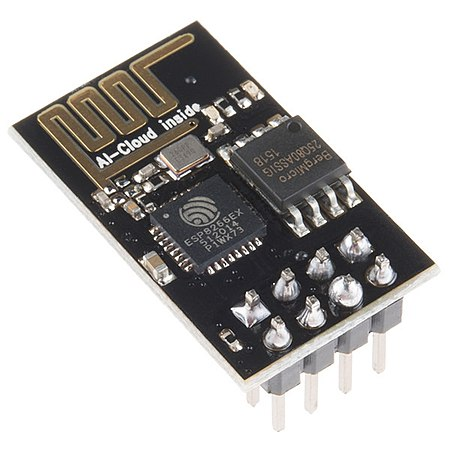
\includegraphics[width=0.17\linewidth]{./img/esp01.jpg}}
	\caption{L'ESP-01 di Ai-Thinker}
	\label{fig:esp01}
\end{figure}

L'Arduino UNO, a differenza di altre board più recenti, non ha il WiFi incorporato perciò bisogna accoppiarlo con uno shield che gli permette di avere quella funzionalità necessaria per un progetto IoT. È stata fatta la scelta di usare l'ESP8266, una famiglia di microchip WiFi a basso costo prodotta da Espressif Systems. Il dispositivo usato in realtà si chiama ESP-01 (Figura \ref{fig:esp01}), è basato sul modulo ESP8266 ed è prodotto da terze parti (Ai-Thinker). Questo piccolo modulo permette a microcontrollori di connettersi alla rete WiFi per fare semplici chiamate HTTP.
Tra le varie caratteristiche vengono elencate le più interessanti:

\begin{itemize}
	\item basso costo e molto compatto;
	\item antenna incorporata nel PCB;
	\item 512 KB flash memory su cui caricare il programma;
	\item 80 KB user data RAM;
	\item può essere usato sia come Station (il caso in questione) che come Access Point;
	\item implementa la funzione Deep Sleep per evitare il consumo eccessivo durante l'inattività;
	\item può essere programmato attraverso l'IDE di Arduino;
	\item implementa il protocollo IEEE 802.11 b/g/n (ovvero WiFi).
\end{itemize}
Il pinout e le funzioni dei pin si trovano rispettivamente nella Figura \ref{fig:esp_pinout_img} e nella Tabella \ref{tab:esp01_pinout}. 

L'ESP-01 va alimentato a una tensione di 3.3V e, secondo \cite{esp_ds}, potrebbe richiedere anche fino a 170mA di corrente perciò non si può alimentare direttamente dal pin 3V3 dell'Arduino perchè non eroga abbastanza corrente (max 50 mA secondo le specificazioni in \cite{uno_specs}). Per questo motivo è stato usato il pin 5V dell'Arduino collegato ad un regolatore di tensione chiamato LM1117 (datasheet: \url{http://www.ti.com/lit/ds/symlink/lm1117.pdf}). 
Il circuito si può trovare nella Figura \ref{fig:esp_uno}.

\vspace{\baselineskip}
\begin{minipage}{\textwidth}
	\begin{minipage}[b]{0.35\textwidth}
		\centering{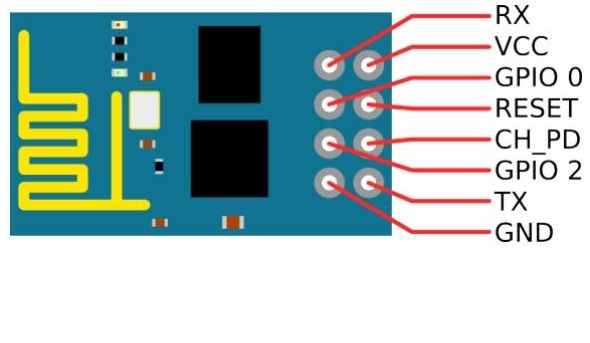
\includegraphics[width=1\linewidth]{./img/esp_pinout_img.jpg}}	
		\captionof{figure}{ESP-01 Pinout}
		\label{fig:esp_pinout_img}
	\end{minipage}
	\hfill
	\begin{minipage}[b]{0.65\textwidth}
		\centering
		\begin{tabular}{l|l}
			\textbf{Pin} & \textbf{Funzione del pin} \\
			\hline
			1 & RX (Receive data bit) \\
			2 & GPIO0 (General Purpose Input/Output Pin) \\
			3 & GPIO2 (General Purpose Input/Output Pin) \\
			4 & GND \\
			5 & VCC (+3.3V) \\
			6 & RST (Reset chip) \\
			7 & CH\_PD (Chip power-down) \\
			8 & TX (Transmit data bit) \\
		\end{tabular}
		\captionof{table}{Funzioni dei pin dell'ESP-01}
		\label{tab:esp01_pinout}
	\end{minipage}
\end{minipage}
\vspace{\baselineskip}

\begin{figure}[H]
	\center{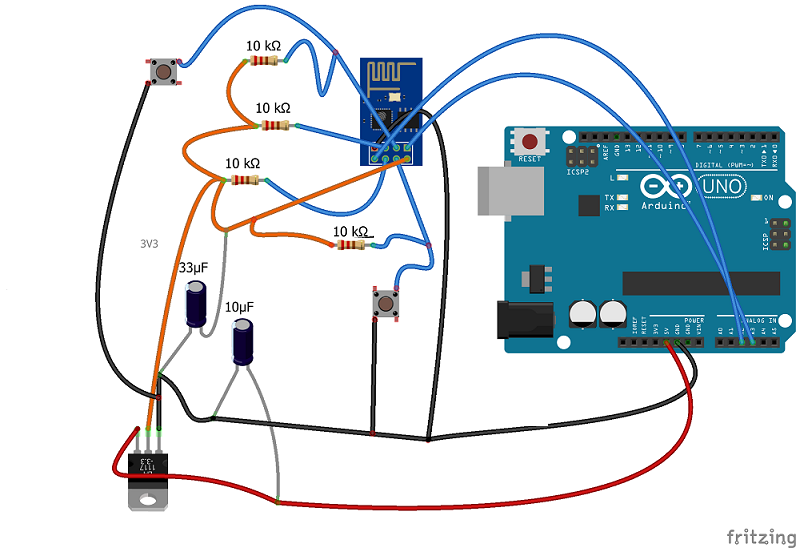
\includegraphics[width=0.75\linewidth]{./img/esp_uno.png}}
	\caption{ESP-01 e Arduino UNO}
	\label{fig:esp_uno}
\end{figure}

Il dispositivo viene pre-programmato con il firmware AT  (\cite{at_fw}) ma è possibile programmarlo anche con il codice proprio mettendolo in modalità di programmazione (vedere la Tabella \ref{tab:esp01_modes}) utilizzando l'IDE di Arduino (Listato \ref{lst:esp01_setup}).

\begin{table}[H]
	\begin{center}
		\begin{tabular}{l|l} 
			\textbf{GPIO-0} & \textbf{Modalità} \\
			\hline
			GND & Flash mode (modalità programmazione) \\
			VCC & Normal mode (il chip esegue il codice caricato) \\
		\end{tabular}
		\caption{Modalità di funzionamento dell'ESP-01}
		\label{tab:esp01_modes}
	\end{center}
\end{table}
\begin{lstlisting}[caption={Riprogrammazione dell'ESP-01 con il codice proprio. All'accensione, il dispositivo non fa altro che connettersi alla rete WiFi locale. Per poter fare ciò, è stata utilizzata una libreria molto bene documentata (\url{https://arduino-esp8266.readthedocs.io/en/latest/esp8266wifi/readme.html})}, label={lst:esp01_setup}]
#include <ESP8266WiFi.h>
#include <ESP8266HTTPClient.h>
#include "wifi_secrets.h"

const char* ssid = SECRET_SSID;
const char* password = SECRET_PASS;

void setup() {
	Serial.begin(9600);
	WiFi.begin(ssid, password);
	Serial.print("Connecting");
	while (WiFi.status() != WL_CONNECTED) {
		delay(1000);
		Serial.print(".");
	}
	Serial.println("\nConnected");
}
\end{lstlisting}
Dopo aver effettuato la connessione, l'ESP-01 si mette in ascolto sulla porta seriale per dati in arrivo dall'Arduino per poi eseguire varie funzioni in base alla richiesta (Listato \ref{lst:esp01_listen}).

\noindent L'Arduino è programmato per mandare 2 tipi di richieste:

\begin{itemize}
	\item \textquotedblleft{} check \textquotedblright{} per quando deve inoltrare all'ESP-01 il codice del tag per la verifica (Listato \ref{lst:uno_checkCardSerial})
	\item \textquotedblleft{} log \textquotedblright{} per quando deve inoltrare all'ESP-01 un log (Listato \ref{lst:uno_sendLog})
\end{itemize}

\pagebreak 

\begin{lstlisting}[caption={L'ESP-01 si mette in ascolto sulla porta seriale collegata all'Arduino. Esso chiama la funzione corretta in base al formato della stringa ricevuta.}, label={lst:esp01_listen}]
void loop() {
	if ( WiFi.status() == WL_CONNECTED ) {
		if ( Serial.available() ) {
		String from_arduinoJSON = Serial.readString();
			if (from_arduinoJSON.startsWith("check")) {
				checkTessera(from_arduinoJSON.substring(5));
			}
			else if (from_arduinoJSON.startsWith("log")) {
				sendLog(from_arduinoJSON.substring(3));
			}
		}
	}
}
\end{lstlisting}
\begin{lstlisting}[caption={L'Arduino manda all'ESP-01 il seriale della tessera in formato JSON e aspetta la risposta con lo status code. Se statusCode = 200 allora mette la variabile allowed a \textquotedblleft{} true \textquotedblright{}. La funzione printBodyToESP si può vedere nel Listato \ref{lst:uno_printBodyToESP} }, label={lst:uno_checkCardSerial}]
boolean checkCard(String serial) {
	boolean allowed = false;
	String bodyJSON = "check{\"seriale\":\"" + serial + "\"}";
	int statusCode = printBodyToESP(bodyJSON);
	switch (statusCode) {
		case 200:
			sendLogTessera(serial);
			allowed = true;
			break;
		... // altri casi
		}
	return allowed;
}
\end{lstlisting}	
\begin{lstlisting}[caption={L'Arduino manda all'ESP-01 il log in formato JSON e aspetta la risposta con lo status code. La funzione printBodyToESP si può vedere nel Listato \ref{lst:uno_printBodyToESP}.}, label={lst:uno_sendLog}]
void sendLog(String tipo) {
	String date = getCurrentFormattedDate();
	String bodyJSON = "log{\"data\":\"";
	bodyJSON.concat(date);
	bodyJSON.concat("Z\",\"tipo\":\"" + tipo + "\"}\0");
	printBodyToESP(bodyJSON);
}
\end{lstlisting}

\noindent In base alla richiesta vengono attivate 2 funzioni diverse:
\begin{itemize}
	\item una per mandare la verifica del tag al server tramite una chiamata HTTP (Listato \ref{lst:esp_checkTessera});
	\item una per mandare il log al server tramite una chiamata HTTP (Listato \ref{lst:esp_sendLog}).
	
\begin{lstlisting}[caption={L'ESP-01 manda una richiesta POST all'endpoint specificato. Il corpo della richiesta è in formato JSON e include il seriale e il tipo della tessera che si vuole verificare.}, label={lst:esp_checkTessera}, xleftmargin=\dimexpr-\leftmargini]
void checkTessera(String tesseraJSON) {
	HTTPClient http;
	http.begin("http://192.168.1.71:3000/api/tessere/check");
	http.addHeader("Content-Type", "text/plain");
	int statusCode = http.POST(tesseraJSON);
	Serial.print(String(statusCode)); // invia all'Arduino
	http.end();
}
\end{lstlisting}
\begin{lstlisting}[caption={L'ESP-01 manda una richiesta POST all'endpoint specificato. Il corpo della richiesta è in formato JSON e rappresenta il log.}, label={lst:esp_sendLog}, xleftmargin=\dimexpr-\leftmargini]
void sendLog(String logJSON) {
	HTTPClient http;
	http.begin("http://192.168.1.71:3000/api/logs/add");
	http.addHeader("Content-Type", "text/plain");
	int statusCode = http.POST(logJSON);
	Serial.print(String(statusCode)); // invia all'Arduino
	http.end();
}
\end{lstlisting}

\end{itemize}

\subsection{Comunicazione tra l'Arduino UNO e l'ESP-01 }

L'Arduino UNO è programmato per comunicare con l'ESP-01 tramite SoftwareSerial (\cite{softwareserial_lib}), una libreria che replica, per via software, le funzionalità della comunicazione seriale hardware (pin 0 e 1 nell'Arduino UNO) anche su altri pin digitali. Un esempio di codice per il setup della comunicazione seriale tra l'ESP-01 e l'Arduino UNO tramite SoftwareSerial si trova nel Listato \ref{lst:uno_ss_setup}
\begin{lstlisting}[caption={Inizializzazione della comunicazione seriale tra Arduino UNO e ESP-01}, label={lst:uno_ss_setup}]
SoftwareSerial ESP(16, 17);

void arduinoEspSerialSetup() {
	ESP.begin(9600);
}
\end{lstlisting}

\noindent Un esempio di utilizzo di SoftwareSerial si può trovare nel Listato (\ref{lst:uno_printBodyToESP}).
\begin{lstlisting}[caption={La funzione printBodyToESP. Essa manda all'ESP-01 (tramite l'oggetto SoftwareSerial) la stringa ricevuta tra gli argomenti e poi aspetta per la risposta. Dopo aver ricevuto la risposta restituisce statusCode.}, label={lst:uno_printBodyToESP}]
int printBodyToESP(String bodyJSON) {
	int statusCode;
	ESP.print(bodyJSON); // manda oggetto all'ESP
	delay(100);
	uint32_t lastMillis = millis();
	while ( !ESP.available() ) {
		// se passano 5 secondi senza risposta, break (per evitare loop)
		if ( !checkTimeout(lastMillis) ) break;
	}
	// se arriva qua abbiamo lo status code
	statusCode = uint32_t(ESP.parseInt()); // cast al tipo uint32
	return statusCode;
}

boolean checkTimeout(uint32_t lastMillis) {
	// espTimeoutInterval = 5000
	if ( (millis() - lastMillis) < espTimeoutInterval ) return true;
	else return false;
}
\end{lstlisting}

Come si è visto precedentemente, l'Arduino inoltra all'ESP-01 delle stringhe che sono quasi in formato JSON: prima dell'oggetto JSON c'è un'altra stringa usata per identificare la funzione voluta (e.g$.$ \textquotedblleft{} check\{object\} \textquotedblright{} e \textquotedblleft{} log\{object\} \textquotedblright{}). L'ESP-01 poi filtra questi dettagli non più necessari e chiama la funzione richiesta.
 Viene presentata la sequenza completa degli eventi per la verifica di un tag:

\begin{enumerate}[(I)]
	\item L'utente avvicina il tag al lettore RFID;
	\item L'Arduino legge il seriale del tag e chiama \textquotedblleft{} checkCard(serial) \textquotedblright{} (Listato \ref{lst:uno_checkCardSerial}). Questa funzione manda una stringa in formato \textquotedblleft{} quasi-JSON \textquotedblright{} all'ESP-01;
	\item L'ESP-01 riceve questa stringa. Esso filtra l'informazione non più necessaria e chiama \textquotedblleft{} checkTessera(tessera) \textquotedblright{} (Listato \ref{lst:esp01_listen});
	\item La funzione eseguita manda l'oggetto JSON al server e aspetta una risposta con lo status code. Dopo aver ricevuto la risposta, esso inoltra lo status code all'Arduino tramite la porta seriale (Listato \ref{lst:esp_checkTessera});
	\item L'Arduino prende una decisione in base allo status code: se 200 allora il tag è accettato e apre la porta, altrimenti viene rifiutato.
\end{enumerate}
Segue un diagramma delle sequenze per il caso in cui la tessera è stata trovata nel database.

\vspace*{20px}

\noindent\begin{tikzpicture}
	\centering
	\footnotesize
	\draw [line width=0.5mm](-11.5,0)--(-11.5,-9) (-8,0)--(-8,-9) (-4.5,0)--(-4.5,-9) (-1.,0)--(-1,-9) (2.5, 0)--(2.5,-9);
	\node at (-11.5,.3) {\normalsize{\textbf{Utente}}};
	\node at (-8,.3) {\normalsize{\textbf{Arduino}}};
	\node at (-4.5,.3) {\normalsize{\textbf{ESP}}};
	\node at (-1,.3) {\normalsize{\textbf{Server}}};
	\node at (2.5,.3) {\normalsize{\textbf{Database}}};
	\draw[->, line width=0.5mm] (-11.5,-1) -- node[midway,above] {\emph{checkCard()}} (-8,-1);
	\draw[->, line width=0.5mm] (-8,-2) -- node[midway,above] {\emph{printBodyToESP()}} (-4.5,-2);
	\draw[->, line width=0.5mm] (-4.5,-3) -- node[midway,above] {\scriptsize{\emph{POST /api/tessere/check}}} (-1,-3);
	\draw[->, line width=0.5mm] (-1,-4) -- node[midway,above] {\emph{findAllowedCard()}} (2.5,-4);
	\draw[dashed, <-, line width=0.5mm] (-1,-5) -- node[midway,above] {\emph{success: found}} (2.5,-5);
	\draw[dashed, <-, line width=0.5mm] (-4.5,-6) -- node[midway,above] {\emph{statusCode = 200}} (-1,-6);
	\draw[<-, line width=0.5mm] (-8,-7) -- node[midway,above] {\emph{print(statusCode)}} (-4.5,-7);
	\draw[<-, line width=0.5mm] (-11.5,-8) -- node[midway,above] {\emph{openDoor()}} (-8,-8);
\end{tikzpicture}

\vspace*{20px}

\noindent Come si può vedere dalla sequenza degli eventi, l'ESP-01 non è altro che un intermediario tra l'Arduino e il server.

%
\section{Protocolli di comunicazione tra dispositivi}
%

%
\subsection{I$^2$C}\label{sec:i2c}
%

\begin{figure}[H]
	\center{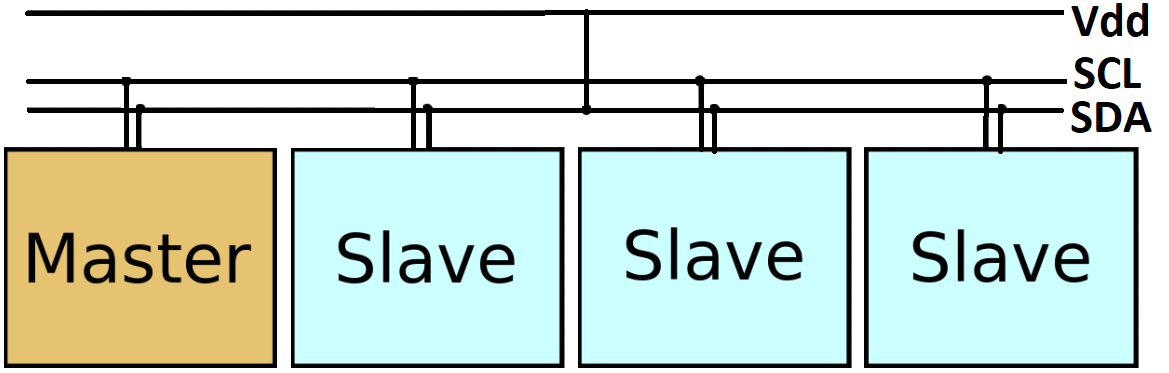
\includegraphics[width=0.6\linewidth]{./img/i2c_bus.png}}
	\caption{I$^2$C Bus}
	\label{fig:i2c_bus}
\end{figure}

\emph{Inter-Integrated Circuit} (I$^2$C) è un protocollo seriale a due vie inventato dalla NXP per far comunicare tra di loro dispositivi come microcontrollori, memorie EEPROM, dispositivi di input/output ecc. È un protocollo creato per la comunicazione sincrona e a breve distanza tra dispositivi chiamati dispositivi master e slave (Figura \ref{fig:i2c_bus}): 

\begin{itemize}
	\item lo slave è un dispositivo che riceve i comandi dal master. Ogni slave ha un indirizzo (deve essere unico all'interno del sistema) normalmente specificato nel datasheet (e.g$.$ 0x27 per il display LCD 16x2 con il backpack PCF8574) attraverso il quale viene indirizzato dal master;
	\item il master non ha bisogno di un indirizzo ed è quello che genera il clock (per via di SCL). Il suo compito è di fare partire la comunicazione con i slave e inviare comandi di lettura/scrittura. Un sistema può avere più dispositivi master.
\end{itemize}
I$^2$C è un protocollo a due vie perchè utilizza due linee bidirezionali:

\begin{itemize}
	\item \emph{Serial Data} (SDA) attraverso il quale viaggiano i dati. I dati vengono trasferiti in \textit{messaggi} che vengono divisi in blocchi di dati a 8 bit. Ogni messaggio inizia con  \textquotedblleft{} Start Condition \textquotedblright{} e finisce con \textquotedblleft{} Stop Condition \textquotedblright{} e ha al suo interno, oltre ai blocchi di dati, l'indirizzo dello slave con cui il master desidera comunicare. Per gestire i comandi di lettura/scrittura è presente un bit di Read/Write. Nel messaggio vengono inclusi anche i bit di ACK/NACK (acknowledge/no-acknowledge) che vengono mandati dal destinatario (lo slave quando si è in modalità \textquotedblleft{} write \textquotedblright{}, il master quando si è in modalità \textquotedblleft{} read \textquotedblright{}) dei blocchi di dati inviati. Un esempio di messaggio si trova nella Figura \ref{fig:i2c_data_bus};
	\item \emph{Serial Clock} (SCL) utilizzato dal master per la sincronizzazione.
\end{itemize}

\begin{figure}[H]
	\center{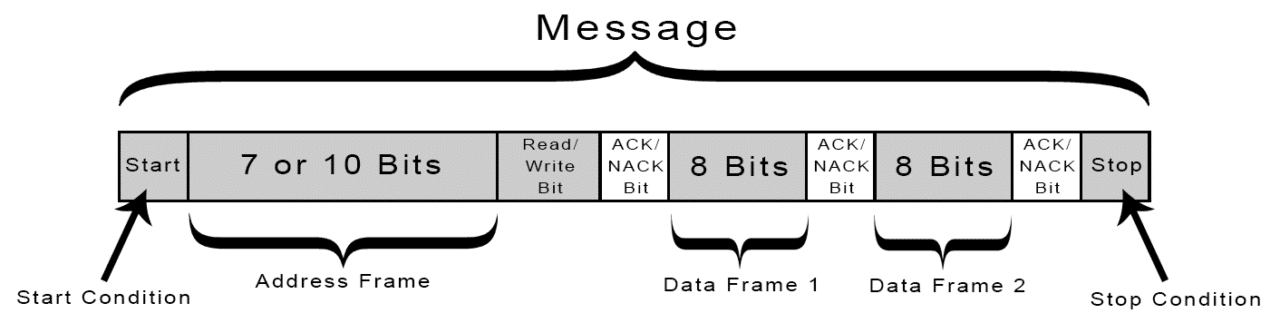
\includegraphics[width=1\linewidth]{./img/i2c_data_bus.png}}
	\caption{Esempio di messaggio inviato sulla linea SDA con il protocollo I$^2$C }
	\label{fig:i2c_data_bus}
\end{figure}


%
\subsection{SPI}\label{sec:spi}
% 

\emph{Serial Peripheral Interface} (SPI) è un protocollo di comunicazione sincrona inventato dalla Motorola e ampiamente utilizzato nei sistemi embedded. Similmente al protocollo I$^2$C, è stato creato per la comunicazione a breve distanza tra un solo dispositivo master e uno o più slave.
SPI è basato su 4 segnali (4-wire bus):

\begin{itemize}
	\item \emph{Serial Clock} (SCLK) utilizzato dal master per la sincronizzazione.
	\item \emph{Master Input Slave Output} (MISO) collegato all'input del master e all'output degli slave. Viene utilizzato dagli slave per inviare dati al master.
	\item \emph{Master Output Slave Input} (MOSI) collegato all'output del master e all'input degli slave. Viene utilizzato dal master per inviare dati allo slave.
	\item \emph{Chip Select} (CS) utilizzato per selezionare lo slave che deve essere abilitato alla comunicazione con il master. Il master può selezionare lo slave con cui vuole parlare semplicemente mettendo a LOW il segnale CS dello slave.
\end{itemize}
Anche se sembrano molto simili, ci sono alcune differenze importanti tra i due protocolli presentati che li rendono adatti per varie applicazioni. Le differenze vengono descritte nella Tabella \ref{tab:i2c_vs_spi}.

\begin{table}[h!]
	\centering
	\def\tabularxcolumn#1{m{#1}}
	\begin{tabularx}{\linewidth}{|L|L|}
		\hline 
		\textbf{I$^2$C} & \textbf{SPI} \\ 
		\hline
		Può avere più master & Può avere un singolo master \\ 
		\hline
		Protocollo a 2 vie & Protocollo a 4 vie (+1 per ogni slave addizionale) \\ 
		\hline
		Velocità fino a 3.4 Mbps in modalità High Speed &  Velocità illimitata (normalmente implementata tra 10 e 100 Mbps) \\ 
		\hline
		Massimo 112 dispositivi con indirizzamento a 7-bit & Limitato dal numero di pin CS del master \\ 
		\hline
		Half-duplex & Full-duplex \\ 
		\hline
	\end{tabularx}
	\caption{I$^2$C vs SPI\cite{i2c_vs_spi}}
	\label{tab:i2c_vs_spi}
\end{table}

%			CAPITOLO 3
\chapter{Sviluppo del sito web}
\label{cap3}
%

\lstset{
	language=Node,
	backgroundcolor=\color{white},
	extendedchars=true,
	basicstyle=\footnotesize\ttfamily,
	showstringspaces=false,
	showspaces=false,
	numbers=left,
	numberstyle=\footnotesize,
	numbersep=9pt,
	tabsize=2,
	breaklines=true,
	showtabs=false,
	captionpos=b
}

\begin{figure}[H]
	\centering{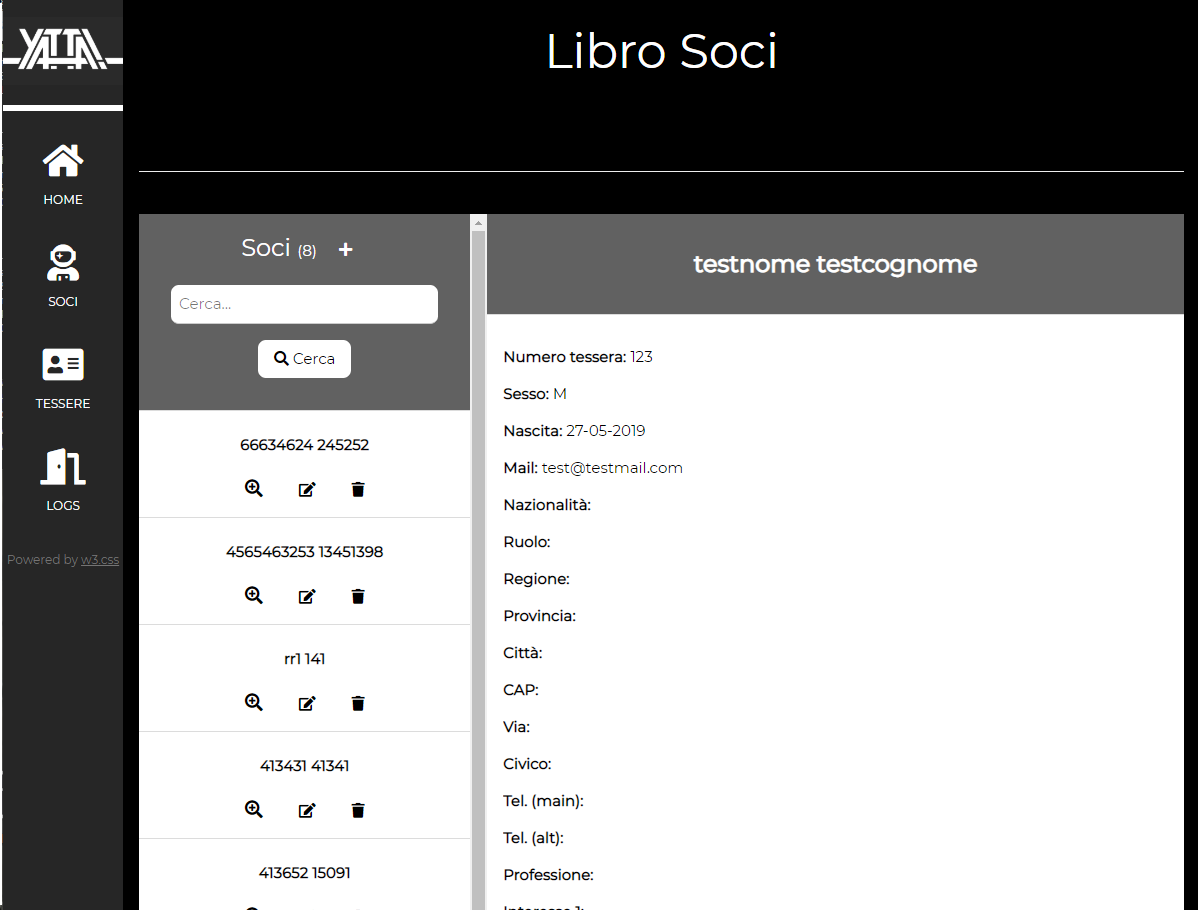
\includegraphics[width=0.9\linewidth]{./img/esempio_libro_soci.png}}
	\caption{Screenshot fatto durante la fase di test del sito web}
	\label{fig:esempio_libro_soci}
\end{figure}

In questo capitolo vengono descritte le tecnologie e le scelte progettuali che hanno portato allo sviluppo dell'interfaccia grafica richiesta dai requisiti per la gestione del database dell'azienda (si veda la sezione \ref{sec:req} \textquotedblleft{} Requisiti del progetto \textquotedblright{}). Nella Figura \ref{fig:esempio_libro_soci} si può vedere un esempio della grafica creata per la gestione del libro soci.

%
\section{Back-End}

In ingegneria del software, il termine back-end rappresenta il lato server di un'applicazione, ovvero un programma che si occupa dei dati dell'applicazione con i quali un utente interagisce indirettamente tramite un'interfaccia. Generalmente il back-end è implementato utilizzando Javascript (Node.js), Python, PHP o Ruby.

\subsection{Tecnologie utilizzate}

\subsubsection*{Node.js}

Node.js (\cite{nodejs}) è un framework open-source che esegue codice JavaScript al di fuori di un browser. È basato sul motore JavaScript V8 di Google ed è stato creato per rendere possibile la creazione di un server utilizzando un linguaggio di programmazione con la stessa sintassi di JavaScript (si parla del paradigma \textquotedblleft{} JavaScript-everywhere \textquotedblright{}). Vengono elencati alcuni vantaggi principali di Node.js

\begin{itemize}
	\item programmazione a eventi (un approccio asincrono): un'azione viene lanciata solo quando succede qualcosa (un evento) e non perforza nell'ordine del codice scritto, aumentando l'efficienza soprattutto nell'ambito di networking dove capita spesso di dover rimanere in attesa di una risposta;
	\item scalabilità del software;
	\item NPM (Node Package Manager): è il più grande ecosistema di librerie open source al mondo. Infatti Node.js ha un enorme quantità disponibile di librerie scritte da altri sviluppatori e possono essere installati facilmente utilizzando NPM;
	\item utilizza lo stesso linguaggio di programmazione degli sviluppatori front-end, perciò è ancora più semplice diventare un full-stack developer grazie al fatto di non dover perforza conoscere linguaggi come Ruby o PHP.
\end{itemize}
L'applicazione utilizza vari moduli di Node.js:

\begin{itemize}
	\item Path (\cite{path}) fornisce alcune utilità nel lavorare con i file e con i percorsi delle directory. L'applicazione usa il modulo per definire una directory statica assoluta per i file dell'applicazione senza dover utilizzare l'intero indirizzo della directory \textquotedblleft{} public \textquotedblright{} (Listato \ref{lst:path});
\begin{lstlisting}[caption={Uso del modulo \emph{path}.}, label={lst:path}, xleftmargin=\dimexpr-\leftmargini]
app.use(express.static(path.join(__dirname, 'public')));
\end{lstlisting}

	\item Express (\cite{express}) è un framework robusto e flessibile che fornisce un insieme di funzioni che facilitano e velocizzano lo sviluppo di applicazioni web con Node.js. L'applicazione fa uso di express per:
	\begin{itemize}
		\item definire delle middleware per rispondere a richieste HTTP e per gestire gli errori. Un esempio di middleware si può trovare nel Listato \ref{lst:middleware}; 
\begin{lstlisting}[caption={Middleware per caricare la pagina \textquotedblleft{} 404.ejs \textquotedblright{} nel caso in cui un utente provi ad accedere ad una pagina non esistente}, label={lst:middleware}, xleftmargin=\dimexpr-\leftmarginii-\leftmargini]
// Catch 404 and forward to error handler

app.use(function(req, res, next) {
	var err = new Error('Not Found');
	err.status = 404;
	next(err);
});
	
app.use(function(err, req, res, next) {

// render the error page
	if (err.status === 404) res.render('404');
	else { // other types of errors
		res.status(err.status || 500);
		res.render('error');
	}
});
\end{lstlisting}

		\item definire una tabella di routing (lista di endpoint accessibili) che viene usata per eseguire diverse azioni in base all'URL e al tipo di richiesta HTTP (esempio nel Listato \ref{lst:routing});
\begin{lstlisting}[caption={Implementazione di un endpoint. Quando viene fatta una richiesta GET all'endpoint \emph{\textquotedblleft{} / \textquotedblright{}} allora, come risposta, l'applicazione invia all'utente un file chiamato \textquotedblleft{} index.ejs \textquotedblright{} (che rappresenta la homepage) che viene poi caricato dal suo browser}, label={lst:routing}, xleftmargin=\dimexpr-\leftmarginii-\leftmargini]
app.get('/', (req, res) => res.render('index'));
\end{lstlisting}

		\item caricare pagine HTML in maniera dinamica passando degli argomenti ai template (e.g. usando un linguaggio di templating chiamato EJS);
		\item si possono creare in maniera semplice e veloce delle API RESTful (si veda la sezione \ref{sec:api});
		\item interfacciarsi con vari database (e.g. MongoDB, MySQL ecc.);
		\item creare un server che ascolta su una porta preimpostata. Per far ciò, express fornisce un'astrazione del modulo \emph{http} di Node.js (esempio nel Listato \ref{lst:server}).
\begin{lstlisting}[caption={Creazione di un server con il modulo \emph{express}}, label={lst:server}, xleftmargin=\dimexpr-\leftmarginii-\leftmargini]
var server = app.listen(port, () => {
	console.log("Listening on port " + server.address().port);
});
\end{lstlisting}   

	\end{itemize}

	\item Body-Parser (\cite{bodyparser}) ispeziona i contenuti delle richieste HTTP. Utile per poter leggere i dati in formato JSON (e non solo). Esempio nel Listato \ref{lst:bodyparser};
\begin{lstlisting}[caption={Uso del modulo body-parser. Vengono definiti dei middleware che analizzano i contenuti delle richieste HTTP.}, label={lst:bodyparser}, xleftmargin=\dimexpr-\leftmargini]
// for parsing
app.use(bodyParser.json()); 
app.use(bodyParser.urlencoded( { extended: true } )); 
app.use(bodyParser.text()); 
\end{lstlisting}

	\item EJS (\cite{ejs}) è un linguaggio di templating che permette di avere dati provenienti dal server direttamente all'interno di documenti HTML. Il codice nel lato server si può vedere nel Listato \ref{lst:ejs_server}, mentre un esempio di utilizzo di EJS nel lato client si può vedere nel Listato \ref{lst:ejs_client};
\begin{lstlisting}[caption={Impostazione del \textquotedblleft{} view engine \textquotedblright{}}, label={lst:ejs_server}, xleftmargin=\dimexpr-\leftmargini]
app.set('view engine', 'ejs');
\end{lstlisting}

	\item Mongoose (\cite{mongoose}) è una libreria di \emph{Object Data Modeling} (ODM) che fornisce un ambiente per la modelizzazione dei dati di MongoDB permettendo la definizione degli oggetti sotto uno schema fortemente tipizzato (si veda la sezione \ref{sec:db} \textquotedblleft{} Database \textquotedblright{}).	
	
\end{itemize}

\pagebreak

\begin{lstlisting}[language=HTML, morekeywords={if, else}, caption={Uso di \emph{EJS} nel lato client. Il codice JavaScript all'interno della pagina HTML è racchiuso tra \textquotedblleft{} $<$\% \%$>$ \textquotedblright{} e l'oggetto \textquotedblleft{} tessere \textquotedblright{} è stato passato dal server in formato JSON. Gli oggetti passati dal server sono racchiusi tra \textquotedblleft{} $<$\%= \%$>$ \textquotedblright{} }, label={lst:ejs_client}]
<% for(var i=0; i<tessere.length; i++) { %>
	<tr class="w3-black tessere-table-mobile">
	<td><%= tessere[i].numero_tessera %></td>
	<td><%= tessere[i].seriale %></td>
	... <!-- altre colonne -->
	<% if ( tessere[i].stato === "ATTIVATA" ) { %>
		<td><div class="green-circle"></div></td>
	<% } else { %>
		<td><div class="red-circle"></div></td>
	<% } %>
	</tr>
<% } %>
\end{lstlisting}

\subsubsection*{MVC}

\begin{figure}[H]
	\center{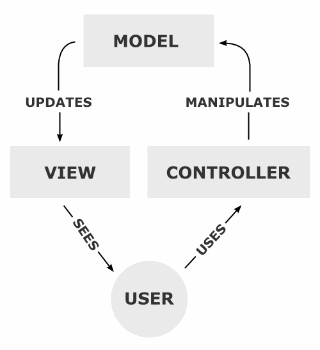
\includegraphics[width=0.35\linewidth]{./img/mvc.png}}
	\caption{Esempio delle interazioni tra i componenti del pattern MVC}
	\label{fig:mvc}
\end{figure}

Per garantire l'indipendenza tra i dati e l'interfaccia, si può modularizzare il codice. La modularizzazione è necessaria soprattutto quando aumenta la complessità di un progetto poichè garantisce che ogni parte sia più comprensibile, facilmente modificabile, scalabile e riutilizzabile.
Il sito web è stato creato sulla base di MVC (Model-View-Controller), un pattern architetturale (Figura \ref{fig:mvc}) che separa un'applicazione in tre principali componenti logici: il modello, la vista e il controller. Ognuno di questi componenti è progettato per gestire diversi aspetti specifici dello sviluppo di un'applicazione:

\begin{itemize}
	\item il modello corrisponde alla struttura e alla logica dei dati dell'applicazione (esempio nel Listato \ref{lst:model});
	\item la vista corrisponde alla logica dell'\emph{User Interface} (UI) dell'applicazione. Rappresenta il modo in cui vengono presentati i dati all'utente (esempio nel Listato \ref{lst:view}); 
	\item il controller accetta l'input dell'utente (e.g. visitare il sito web, cliccare su un pulsante, inviare un modulo ecc.) e lo trasforma in comandi per il modello o per la vista (esempio nel Listato \ref{lst:controller}).
	
\begin{lstlisting}[caption={Creazione del modello dei log con \emph{mongoose}}, label={lst:model}, xleftmargin=\dimexpr-\leftmargini]
var mongoose = require('mongoose');
var Schema = mongoose.Schema;

var LogSchema = new Schema ({
	tipo: { type: String, enum: ["telecomando", "tessera", "keypad"], required: true, lowercase: true, trim: true },
	seriale: { type: String, default: "N/A", uppercase: true, trim: true },
	nome: { type: String, default: "N/A", lowercase: true, trim: true },
	cognome:  { type: String, default: "N/A", lowercase: true, trim: true },
	numero_tessera: { type: String, default: ""},
	data: { type: Date, required: true }
});

/*Tutte le stringhe incluse nell'indice.
*	Permette di cercare l'intero database */

LogSchema.index( { '$**': 'text'}); // full-table search index

module.exports = mongoose.model("Log", LogSchema);
\end{lstlisting}

\pagebreak

\begin{lstlisting}[language=HTML, morekeywords={if, else}, caption={Parte del codice HTML della vista creata per presentare le tessere all'utente}, label={lst:view}, xleftmargin=\dimexpr-\leftmargini]
<table class="w3-table w3-left w3-border w3-centered">
	<thead>
		<tr class="w3-white tessere-table-mobile w3-large">
			<th>Numero tessera</th>
			<th>Seriale</th>
			... <!-- altre colonne -->
		</tr>
	</thead>
	<tbody>
		<% for(var i=0; i<tessere.length; i++) { %>
			<tr class="w3-black tessere-table-mobile">
				<td><%= tessere[i].numero_tessera %></td>
				<td><%= tessere[i].seriale %></td>
				...
			</tr>
	</tbody>
</table>
\end{lstlisting}
\begin{lstlisting}[caption={Parte del codice del controller creato per gestire i comandi relativi ai soci.  Questa funzione, quando viene chiamata, cerca nel database i soci in base al termine inviato tra i parametri e poi carica una pagina con i risultati.}, label={lst:controller}, xleftmargin=\dimexpr-\leftmargini]
exports.fullTableSearch = (req, res) => {
	let searchTerm = req.params.term;
	Socio.
	find( { $text: { $search: searchTerm } } ).
	exec(function(err, soci) {
		if (err) {
			console.error(err);
			return res.status(500).send("Internal Server Error");
		} else return res.render("../views/soci/soci_index", { searched: "true", soci: soci, sociString: JSON.stringify(soci) });
	});
}
\end{lstlisting}
	 
\end{itemize}

\subsection{Database}\label{sec:db}
%
Il \emph{Database Management System} (DBMS) scelto per l'applicazione si chiama MongoDB (\cite{mongodb}). MongoDB è un DBMS open-source e non relazionale (è classificato come un database di tipo NoSQL) ed è orientato ai documenti: al posto delle tipiche tabelle dei database relazionali vengono utilizzati dei documenti in formato JSON (particolarmente BSON, ovvero Binary JSON: una serializzazione codificata in binario di JSON), facilitando quindi l'integrazione dei dati con quasi tutte le applicazioni web (infatti JSON è il formato di dati più utilizzato per lo scambio dei dati in rete).
MongoDB si integra facilmente con Node.js grazie a dei driver creati dagli sviluppatori stessi (\cite{mongodb_driver}). Questi driver, purtroppo, non portano tanta astrazione e sollevano dei problemi per chi non è abituato a un database NoSQL: 
\begin{itemize}
	\item la logica dei dati è diversa rispetto a quella che viene insegnata nei corsi tradizionali di basi di dati perciò potrebbe essere difficile abituarsi (ma, come si vedrà, anche non necessario);
	\item non c'è la possibilità di validare i dati in maniera semplice ma bisogna scrivere del codice che potrebbe essere soggetto a errori;
	\item le query con i driver nativi di MongoDB non sono tanto leggibili e possono diventare molto complesse perchè usano un insieme di operatori (e.g. quello di uguaglianza \textquotedblleft{} \$eq \textquotedblright{}). Esempio:
\begin{lstlisting}
Account.find({ nome: { $eq: 'Andrea' } });
\end{lstlisting}

	\item la manutenzione è resa più complicata per la mancanza di una struttura fissa dei dati.
\end{itemize}

È possibile però avere più astrazione (ad un basso costo di performance) utilizzando Mongoose, una libreria basata sui driver di MongoDB ideata per la modellazione degli oggetti di MongoDB e progettata per funzionare in un ambiente asincrono (come Node.js). Mongoose rende più semplice e immediato l'utilizzo di MongoDB per alcuni motivi:
\begin{itemize}
	\item facilità di apprendimento;
	\item query più semplificate e leggibili (soprattutto quando diventano complesse) grazie al \textquotedblleft{} method chaining \textquotedblright{} di JavaScript. Esempio nel Listato \ref{lst:method_chaining};
	\item fornisce un modo per dare una struttura ai dati grazie alla creazione degli schemi; ogni schema può essere compilato in un modello, ovvero una classe con cui vengono costruiti i documenti con i comportamenti (metodi) e le proprietà (attributi) dello schema dato;
	\item permette di validare i dati all'interno degli schemi (e.g. attributo: \{ type: String, lowercase: true \});
	\item libreria progettata per un ambiente asincrono: è possibile definire delle middleware (pre, post) da chiamare prima o dopo una certa operazione (e.g. di salvataggio). 
\end{itemize}
\begin{lstlisting}[caption={Esempio di query con \emph{mongoose}. Questa funzione cerca nel database dei soci per l'identificatore passato tra i parametri e poi carica la pagina per aggiornare il socio trovato}, label={lst:method_chaining}]
exports.updateSocio = (req, res) => {
	Socio.
	findOne( { _id: req.params.id } ).
	exec( (err, socio) => {
		if (err) {
			console.error(err);
			return res.status(500).send("Internal Server Error");
		} else return res.render("../views/soci/soci_update", { socio: socio });
	});
}
\end{lstlisting}

Come esempio dimostrativo per accedere al database, viene presentata la sequenza degli eventi per aggiungere un log (dopo un accesso con la tessera) all'interno del database e poi visualizzarlo sul sito:
\begin{enumerate}[(I)]
	\item L'ESP-01 manda una richiesta di aggiunta del log all'endpoint \emph{/api/logs/add} del server (Listato \ref{lst:esp_sendLog});
	\item L'applicazione, dopo aver ricevuto una richiesta POST all'endpoint specificato precedentemente, chiama una funzione per gestire la richiesta (Listato \ref{lst:add_log_endpoint});	
\lstset{
	language=Node,
	backgroundcolor=\color{white},
	extendedchars=true,
	basicstyle=\footnotesize\ttfamily,
	showstringspaces=false,
	showspaces=false,
	numbers=left,
	numberstyle=\footnotesize,
	numbersep=9pt,
	tabsize=2,
	breaklines=true,
	showtabs=false,
	captionpos=b
}
\begin{lstlisting}[caption={Endpoint per aggiungere i log}, label={lst:add_log_endpoint}, xleftmargin=\dimexpr-\leftmargini]
app.post('/api/logs/add', logs.addLog);
\end{lstlisting}
	\item La funzione gestisce la richiesta e salva il log nel database (Listato \ref{lst:saveLog});
	\item Il log è visualizzabile sul sito accedendo all'endpoint \emph{/api/logs/view} (la pagina caricata si può vedere nella Figura \ref{fig:logbook})$.$ Il codice eseguito dopo una richiesta GET all'endpoint specificato si può trovare nel Listato \ref{lst:viewLogs}.
	
\end{enumerate}
Il ragionamento per aggiungere i soci e le tessere al database è simile, solo che si può fare direttamente dal sito: il browser manda i form compilati tramite una richiesta POST al server. Per ogni tipo di richiesta diversa, verrà chiamata una funzione specifica per gestirla.

\pagebreak
	
\begin{lstlisting}[caption={Questa funzione aggiunge il log all'interno del database. Il corpo della richiesta POST contiene il log in formato JSON}, label={lst:saveLog}]
exports.addLog = (req, res) => {
	var body = JSON.parse(req.body);
	... // alcune righe di codice per validare i dati
	if (body.tipo === "tessera") { // log con tessera 
		Tessera.
		findOne( { seriale: body.seriale } ). // trova la tessera 
		populate('socio').
		exec( (err, tessera) => {
			if (err) return console.error(err);
			if (tessera) {
				let log = new Log ({
					nome: tessera.socio.nome,
					cognome: tessera.socio.cognome,
					numero_tessera: tessera.numero_tessera,
					seriale: tessera.seriale,
					data: date,
					tipo: body.tipo
				});	
				log.save( (err) => {
					if (err) console.error(err);
					else {
						console.log("Log aggiunto");
						return res.status(200).send();
					}
				});
			} else return res.status(404).send("Not Found");
		});
	} else { ... } // codice per il caso senza tessera
}
\end{lstlisting}

\begin{lstlisting}[caption={Questa funzione viene eseguita quando un browser accede (richiesta GET) all'endpoint \emph{/api/logs/view}}, label={lst:viewLogs}]
exports.viewAllLogs = (req, res) => {
	Log.find( (err, logs) => {
		if (err) {
			console.error(err);
			return res.status(500).send("Internal Server Error");
		} else {
			return res.render("../views/logs/logs_index", { logs: logs });
		}
	});
}
\end{lstlisting}

\begin{figure}[H]
	\centering{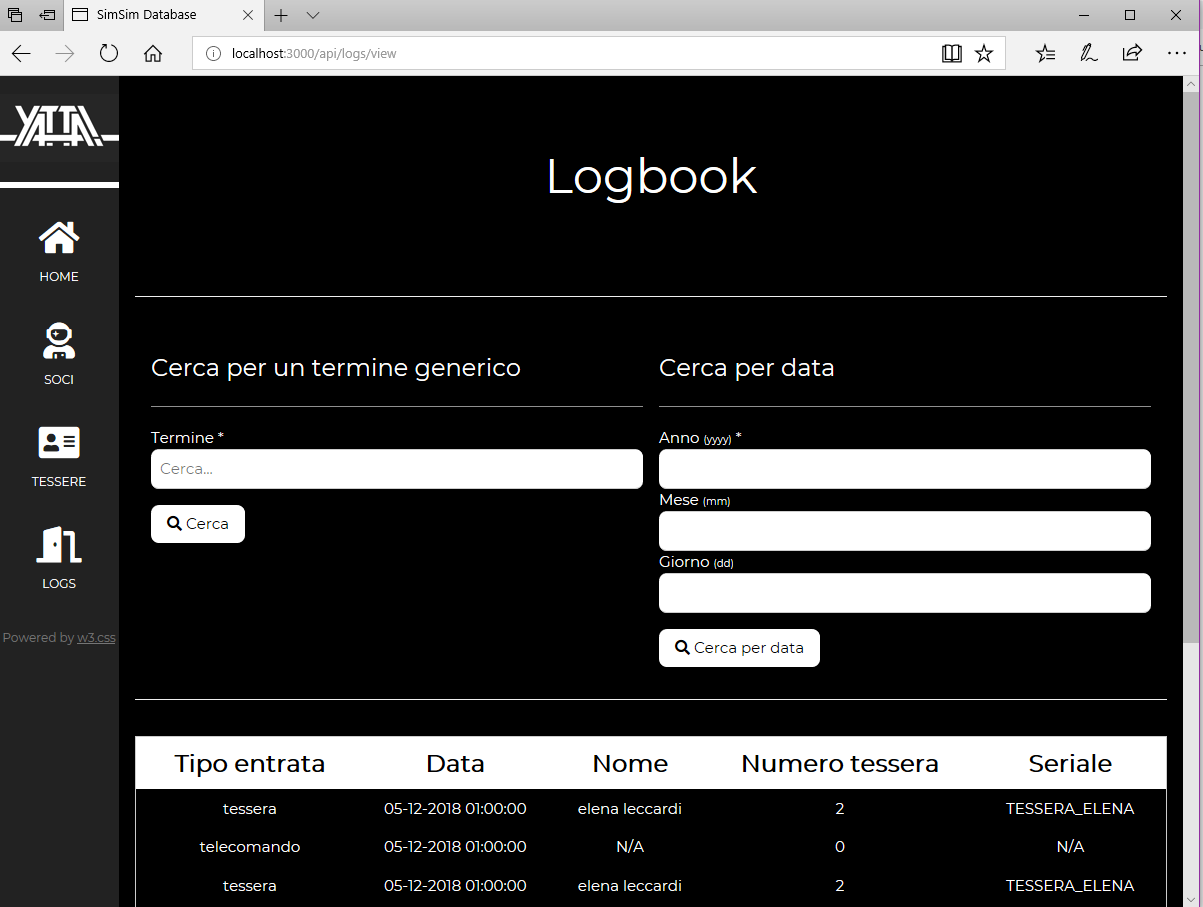
\includegraphics[width=1\linewidth]{./img/logbook.png}}
	\caption{Il logbook dell'azienda}
	\label{fig:logbook}
\end{figure}

\subsection{RESTful API}\label{sec:api}
%
In ambito web, il termine \emph{Application Programming Interface} (API) è utilizzato per rappresentare un insieme di specificazioni per far comunicare tra di loro client (generalmente il browser) e server tramite richieste e risposte HTTP. Vengono specificati e descritti gli endpoint, i tipi di richiesta e risposta (struttura dei dati inviati, messaggi di errore ecc.).
Le API RESTful sono basate su tecnologia \emph{Representational State Transfer} (REST), uno stile architetturale spesso utilizzata nello sviluppo delle applicazioni web. Il concetto più importante in REST è l'esistenza di risorse a cui si possono accedere tramite identificatori univoci chiamati \emph{Uniform Resource Identifier} (URI), ovvero gli endpoint.
Tipicamente le API RESTful sfruttano le chiamate HTTP per dare la possibilità a utenti di leggere (GET), aggiornare (PUT), creare (POST) e rimuovere (DELETE) risorse. 

Un elenco delle API dell'applicazione si può trovare nella Tabella \ref{tab:api}.
Le API sono state testate con Postman (\cite{postman}), un software progettato per lo sviluppo e il testing delle API web. Postman dà la possibilità allo sviluppatore di creare diversi tipi di richieste HTTP da inviare ad un URL e di leggere la risposta ricevuta. Un esempio di utilizzo di Postman si può trovare nella Figura \ref{fig:postman_test}.

\begin{figure}[H]
	\center{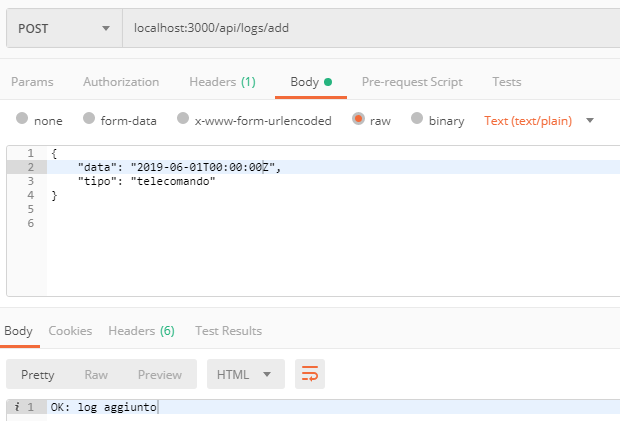
\includegraphics[width=0.9\linewidth]{./img/postman_test.png}}
	\caption{Esempio di testing con Postman dell'endpoint relativo all'aggiunta dei log}
	\label{fig:postman_test}
\end{figure}

\pagebreak

\vspace*{35px} 
\begin{table}[H]
	\scriptsize
	\centering
	\def\tabularxcolumn#1{m{#1}}
	\renewcommand\arraystretch{1.8}
	\renewcommand\tabcolsep{3.0pt}
	\begin{tabularx}{\textwidth}{|L|L|L|L|}
		\hline
		\textbf{Metodo + URI} & \textbf{Parametro} & \textbf{Body} & \textbf{Descrizione} \\
		\hline                              
		GET / & N/A & N/A & Carica la homepage \\ 
		\hline
		GET /api/logs/search/:key & Chiave per la ricerca & N/A 
		& Cerca nel database dei log in base al parametro inviato e carica la pagina con i risultati \\
		\hline
		GET /api/logs/view & N/A & N/A & Carica la pagina con tutti i log \\
		\hline  
		POST /api/logs/add & N/A & Oggetto in formato JSON secondo lo schema Log & Aggiunge un log nel database \\
		\hline
		GET /api/soci/search/:key & Chiave per la ricerca & N/A & Cerca nel database dei soci in base al parametro inviato e carica la pagina con i risultati \\ 
		\hline
		GET /api/soci/view & N/A & N/A & Carica la pagina con tutti i log \\ 
		\hline
		GET /api/soci/create & N/A & N/A & Carica la pagina per creare i soci \\ 
		\hline
		GET /api/soci/update/:id & Chiave identificativa del socio & N/A & Carica la pagina per aggiornare un socio \\ 
		\hline
		POST /api/soci/add & N/A & Oggetto in formato JSON secondo lo schema Socio & Aggiunge un socio nel database \\ 
		\hline
		PUT /api/soci/update/:id & Chiave identificativa del socio & Oggetto in formato JSON secondo lo schema Socio & Aggiorna un socio \\ 
		\hline
		DELETE /api/soci/delete/:id & Chiave identificativa del socio & N/A & Cancella un socio dal database \\ 
		\hline
		GET /api/tessere/view & N/A & N/A & Carica la pagina con tutte le tessere \\ 
		\hline
		POST /api/tessere/check & N/A & Oggetto in formato JSON secondo lo schema Tessera & Verifica se un tag esiste nel database \\
		\hline
		POST /api/tessere/add & N/A & Oggetto in formato JSON secondo lo schema Tessera & Aggiunge una tessera \\ 
		\hline
		PUT /api/tessere/update/:id & Chiave identificativa della tessera & N/A & Cambia lo stato di una tessera (attivata/disattivata) \\ 
		\hline
		DELETE /api/tessere/delete/:id & Chiave identificativa della tessera & N/A & Cancella una tessera dal database \\ 
		\hline
	\end{tabularx}
	\captionsetup{font={footnotesize}}
	\caption{Specificazione delle API dell'applicazione}
	\label{tab:api}
\end{table}

%
\section{Front-End}
%

In ingegneria del software, il termine front-end rappresenta l'interfaccia dell'applicazione, ovvero la parte visibile agli utenti e quella con cui essi interagiscono.

%
\subsection{Tecnologie utilizzate}
%

Per creare il front-end sono stati utilizzati i tipici linguaggi come HTML (per la struttura e il contenuto), CSS (per lo stile) e client-side JavaScript per aggiungere dinamicità al sito (pulsanti, chiamate AJAX ecc.).

%
\subsubsection*{HTML5}
%
\emph{Hyper Text Markup Language} (HTML) è il linguaggio di markup standard nato all'inizio degli anni novanta per la formattazione e impaginazione di documenti progettati per essere visualizzati in un browser. Viene spesso utilizzato insieme ad un linguaggio di stile (CSS) e uno di scripting (JavaScript). L'ultima versione standardizzata dal W3C è HTML 5.1.
I file HTML generati nel progetto hanno l'estensione EJS perchè vengono usati assieme al linguaggio di templating per portare i dati provenienti dal server direttamente nel documento stesso.
%
\subsubsection*{CSS}
%
I documenti HTML sono stilizzati con il linguaggio di stile più diffuso al mondo chiamato \emph{Cascading Style Sheets} (CSS): esso descrive, attraverso delle regole, i modi in cui gli elementi di un documento devono essere presentati e animati nell'interfaccia grafica. Le regole possono essere scritte direttamente nel file HTML, ma ciò crea solo confusione ed è generalmente buona norma avere i file CSS separati e poi importati nel documento (come nel Listato \ref{lst:import_css})
\begin{lstlisting}[language=HTML, caption={Importazione dei file di stile nel documento HTML}, label={lst:import_css}]
<link rel="stylesheet" href="/css/w3.css">
<link rel="stylesheet" href="/css/custom.css">
<link rel="stylesheet" href="/css/font-awesome.min.css">
\end{lstlisting}

Normalmente gli sviluppatori non scrivono le proprie regole (è un lavoro molto lungo e per fare una cosa bella serve tanta esperienza in web design) ma trovano dei template (esistono sia gratis che a pagamento) da utilizzare. In questo caso è stato utilizzato un template (\cite{w3css_template}) di W3.CSS scelto dal tutor aziendale. W3.CSS è un framework moderno, semplice, veloce e gratis che supporta un design \textquotedblleft{} mobile first \textquotedblright{} che aiuta lo sviluppatore a creare siti web moderni e responsivi. Il vantaggio di un sito responsivo è che è progettato per rispondere automaticamente a tutti i tipi di dispositivi utilizzati per visualizzarlo (e.g. desktop, mobile, tablet). Questo approccio viene implementato sfruttando le caratteristiche delle \emph{media queries} (Listato \ref{lst:media_query}).
\begin{lstlisting}[morekeywords={ @media, max-width, px, width, height, !important}, caption={Esempio di \emph{media query}}, label={lst:media_query}]
@media (max-width:768px)
{
	.red-circle
	{
		width: 25px!important;
		height: 25px!important;
	}
	
	.green-circle
	{
		width: 25px!important;
		height: 25px!important;
	}
}
\end{lstlisting}
Inoltre è stato utilizzato \emph{Font Awesome}, un toolkit di icone distribuito sotto licenze libere (CC BY 4.0 e MIT).
%
\subsubsection*{JavaScript}
%
JavaScript è un linguaggio di programmazione introdotto nel 1995 con lo scopo di aggiungere programmi all'interno di siti web sul browser Netscape Navigator. Il linguaggio è stato adottato da quasi tutti gli altri browser esistenti (è stato anche standardizzato sotto il nome di ECMAScript) e ha reso possibile avere applicazioni web moderne con cui un utente può interagire direttamente senza dover ricaricare la pagina\cite{eloquent_javascript}. È un linguaggio molto evoluto e studiato nel tempo e ora si definisce come un linguaggio di scripting client-side (ma non solo, come si è visto con Node.js) eseguito dai browser. Il codice JavaScript può essere scritto all'interno di qualsiasi documento, ma è buona norma avere i file con estensione .js separati e poi inclusi alla fine del documento (per far sì che tutti gli elementi vengano caricati dal browser), come nel Listato \ref{lst:import_javascript}.
\begin{lstlisting}[language=HTML, caption={Importazione dei file .js nel documento HTML}, label={lst:import_javascript}]
<script type="text/javascript" src=/js/jquery-3.3.1.min.js></script>
<script type="text/javascript" src=/js/forms.js></script>
<script type="text/javascript" src=/js/buttons.js></script>
<script type="text/javascript" src=/js/dettagliSoci.js></script>
\end{lstlisting}

JavaScript è un linguaggio che utilizza un singolo thread (organizza l'esecuzione in un'unica pila chiamata \emph{call stack}) e segue il paradigma della programmazione a eventi, perciò è possibile costruire un comportamento non bloccante. Il motore JavaScript crea una coda di eventi (che possono essere operazioni di I/O, richieste di rete, chiamate di WebWorker, funzioni inserite in timer ecc.) che, al verificarsi di un evento, possono modificare l'ordine di esecuzione sequenziale del codice. Si prenda come esempio la funzione nel Listato \ref{lst:hello_world}.
\begin{lstlisting}[language=JavaScript, morekeywords={ alert }, caption={Programmazione a eventi: funzione che scrive \textquotedblleft{} Hello World \textquotedblright{} ogni 3 secondi (in questo caso l'evento è rappresentato dal timer)},label={lst:hello_world}]
function myFunction() {
	setInterval(function() { 
		alert("Hello World"); 
	}, 3000);
}
\end{lstlisting}

JavaScript interagisce con il browser attraverso il \emph{Document Object Model} (DOM) della pagina HTML. Il DOM è stato standardizzato dalla W3C e viene creato dal browser dopo che una pagina è stata caricata. Esso segue un modello gerarchico di oggetti (Figura \ref{fig:dom}) che possono essere manipolati dagli script dando la possibilità di aggiornare dinamicamente il contenuto, la struttura e lo stile dei documenti. Grazie al DOM è possibile accedere agli elementi (e loro proprietà, metodi ed eventi) delle pagine HTML.

Nel progetto è stato utilizzato \emph{jQuery} (\cite{jquery}), una libreria molto diffusa (ormai di meno rispetto a qualche anno fa dato che ora ci sono altre scelte più moderne come React.js, Vue.js e Angular.js) di JavaScript proposta a ridurre e semplificare il codice per lo sviluppo del front-end. Esistono tanti test di benchmark per quanto riguarda la prestazione di jQuery rispetto al \textquotedblleft{} vanilla JavaScript \textquotedblright{}. Secondo Marco Trombino, uno sviluppatore di front-end che ha testato una funzione che inserisce 10,000 elementi nuovi con una classe all'interno di un altro elemento, è stato rilevato che jQuery è molto meno performante rispetto al JavaScript normale: \textit{\textquotedblleft{} As we could have expected Vanilla performed the task in 18,99 ms, whereas jQuery did it in 195,89 ms. Ten times faster. \textquotedblright{}}\cite{jquery}. Nonostante ciò, la scelta di usare jQuery è stata fatta poichè il progetto non è di grosse dimensioni e il costo da pagare per la prestazione non è notevole; in cambio il codice scritto è più corto e semplificato. 

Un elemento molto importante di JavaScript di cui ne vale la pena parlare è la tecnica \emph{Asynchronous JavaScript and XML} (AJAX). AJAX è una tecnica molto utilizzata in ambito web che consente l'aggiornamento dinamico di una pagina web senza dover ricaricarla: lo scambio dei dati tra client e server (e.g. invio di un form) avviene nel background.
\begin{figure}[H]
	\center{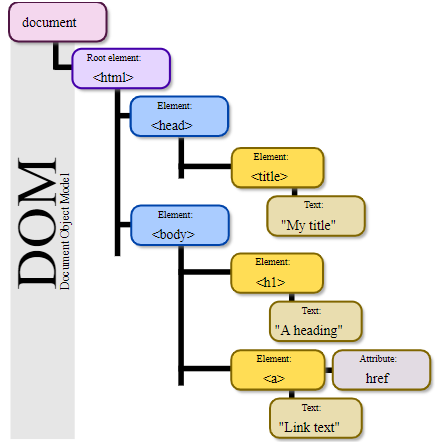
\includegraphics[width=0.6\linewidth]{./img/dom.png}}
	\caption{Esempio di gerarchia del DOM in un documento HTML. Immagine sotto licenza CC BY-SA 3.0. Autore: Birger Eriksson. Link: \url{https://commons.wikimedia.org/wiki/File:DOM-model.svg}}
	\label{fig:dom}
\end{figure}

\noindent Alcuni vantaggi dovuti al fatto di non dover ricaricare la pagina sono: 
 
\begin{itemize}
	\item velocità ed efficienza: il traffico sul server viene ridotto grazie al fatto di dover scambiare solo i dati necessari anzichè l'intera pagina;
	\item sito più responsivo: è possibile aggiornare solo una parte della pagina;
	\item utilizzo minore della larghezza di banda sia dal lato del client che dal lato del server;
	\item validazione istantanea dei form.
\end{itemize}
Tutto ciò è possibile grazie all'utilizzo di un oggetto chiamato XMLHttpRequest che può comunicare con il server per mandare e ricevere dati in vari formati quali JSON, XML, HTML e file di testo in maniera asincrona. Un esempio che descrive l'utilizzo di AJAX si può vedere nel Listato \ref{lst:delete_socio}.
\pagebreak
\begin{lstlisting}[language=JavaScript, morekeywords={ confirm, $, alert }, caption={Tecnica AJAX. La funzione, dopo aver premuto il pulsante per rimuovere un socio, manda una richiesta (nel background) del tipo  \textquotedblleft{} DELETE \textquotedblright{} all'endpoint \emph{/api/soci/delete/} con l'ID del socio che si desidera cancellare}, label={lst:delete_socio}]
const rimuoviSocioButton = $(".w3-btn.w3-round.rimuoviSocioButton");

rimuoviSocioButton.on('click', function(e) {
	e.preventDefault();
	if (!confirm("Rimuovere il socio?")) return false;
	let xHttp = new XMLHttpRequest();
	xHttp.onreadystatechange = function() {
		if (xHttp.readyState == 4) {
			if (xHttp.status === 200) alert("Socio rimosso dal database");
			else alert("Problema: Status Code = " + xHttp.status);
		}
	};
	let id = this.value;
	xHttp.open("DELETE", "/api/soci/delete/" + id, true);
	xHttp.send();
});
\end{lstlisting}

%
% 
%			CAPITOLO 4: Analisi del progetto
\chapter{Analisi e Conclusioni}
\label{cap4}
%

\section{Problemi affrontati}
%

In seguito vengono descritti alcuni problemi affrontati durante lo sviluppo del progetto e le soluzioni adottate per superarli.

%
\subsection{Incompatibilità tra Raspbian e le ultime versioni di MongoDB}
%
Durante lo sviluppo del progetto ho scoperto che Raspbian, il sistema operativo progettato per il Raspberry Pi, in realtà non è stato ancora aggiornato per essere un sistema operativo a 64 bit, perciò non poteva sfruttare al meglio l'architettura a 64 bit del Raspberry Pi 3B+.
L'ultima versione di MongoDB che può essere installata su Raspbian è v2.4 (rilasciato nel 2013) e ha alcuni problemi a connettersi con le ultime versioni di Node.js. Inoltre la versione di MongoDB installata su Raspbian è stata progettata per un'architettura a 32 bit, limitata, per motivi tecnici, a 2GB di dati\cite{mongodb_32bit_limitations}.
Come soluzione a questo problema, è stato installato un sistema operativo chiamato openSUSE Tumbleweed (\cite{tumbleweed}) che funziona su architetture ARMv8 a 64 bit. Ci sono alcune inconvenienze tra cui la più notevole è la minore prestazione offerta dalla Raspberry Pi, però non ha creato grossi problemi e il server è abbastanza responsivo ai comandi. 

%
\subsection{Problema di sicurezza all'interno della rete locale}
%
Siccome non è stato sviluppato un sistema di login per il sito web (per questioni di tempo), qualsiasi persona connessa alla rete locale dell'azienda poteva accedere al sito e vedere/modificare le informazioni del database, perciò è stato deciso di utilizzare un router dedicato per creare una rete LAN privata (e priva di connessione Internet dato che il server risiede in locale) per il progetto. All'ESP-01 e Raspberry Pi sono stati assegnati indirizzi IP statici per far sì che, una volta configurati, riescano a comunicare tra di loro. L'amministratore, per poter accedere al sito web, deve semplicemente connettersi alla rete LAN (solo lui conosce SSID e password).


%
\subsection{Disattivazione delle tessere dei soci non più iscritti}
%

L'ingresso nello spazio di Yatta è regolato da un tesseramento. Ogni anno, a fine Gennaio, tutte le tessere che non sono state rinnovate vengono disattivate: questo significa che devono essere disattivate automaticamente anche nel database.
Per fare questo lavoro è stato creato uno scheduler dal lato del server (Listato \ref{lst:scheduler}).
\begin{lstlisting}[caption={Implementazione di uno scheduler che disattiva automaticamente le tessere non rinnovate. Questa funzione viene eseguita una volta all'anno e disattiva tutte le tessere ancora attivate e non iscritte all'anno corrente.}, label={lst:scheduler}]
var Tessera = require('../models/tessera.model.js');
var schedule = require('node-schedule');

var rule = new schedule.RecurrenceRule();
rule.month = 0; // gennaio - 0
rule.date = 30; // giorno 30
rule.hour = 18; // ore 18
rule.minute = 30; // minuti 30
rule.second = 0; // secondi 0

// e.g. a Gennaio 2019 disattiva le tessere con ultimo_rinnovo<=2018
var j = schedule.scheduleJob(rule, function(){
	nowYear = new Date().getFullYear();
	Tessera.find( (err, tessere) => {
		if (err) console.error(err);
		else {
			for (i=0; i<tessere.length; i++) {
				tessera = tessere[i];
				if ( (nowYear !== tessera.ultimo_rinnovo.getFullYear()) 
				     && (tessera.stato == "ATTIVATA") ) {
					tessera.stato="DISATTIVATA";
					tessera.save( (err, tessera) => {
						if (err) console.error(err);
						else console.log(tessera.numero_tessera + " bloccata");
					});
				}
			}
		}
	});
});
\end{lstlisting}

%
\section{Possibili miglioramenti}
%

Ci sono alcuni possibili miglioramenti che sono stati tralasciati per questioni di tempo ma che potrebbero comunque essere implementati in future versioni:

\begin{itemize}
	\item sistema di login sul sito web per l'amministratore: con questo sistema si può eliminare il router dedicato alla rete LAN dato che solo l'amministratore può fare il login; 
	\item orario di lavoro: è possibile far sì che l'Arduino sia attivo soltanto durante la fascia oraria 9-18 in cui c'è qualcuno in sede. Questo serve per evitare che qualcuno riesca ad aprire la porta in qualsiasi modo (e.g. telecomando o tessera rubata) al di fuori della fascia oraria;
	\item sensore di rilevamento: l'Arduino è stato programmato per chiudere la porta dopo un certo intervallo di tempo. È possibile aggiungere un sensore per il rilevamento delle persone per fare in modo che la porta venga chiusa solo quando non ci sono più persone nella vicinanza;
	\item videocamera: è possibile aggiungere una videocamera connessa alla stessa rete locale che trasmette il video direttamente al server. Questo video potrebbe facilmente essere visualizzabile direttamente sul sito;
	\item sistema di allarme: si potrebbe installare un sistema di allarme per quando la porta viene aperta forzatamente durante la fascia oraria di inattività. Questo sistema di allarme può essere disabilitato manualmente tramite una password nel caso in cui l'amministratore dovesse usare la porta in quell fascia oraria.
\end{itemize}

%
\section{Conclusioni}
%

Il frutto di questo progetto è stato il prototipo di un sistema di controllo accessi IoT (con il server in locale) per l'azienda ospitante del tirocinio. Sono stati presentati i dettagli necessari per capire tutti i componenti e i passaggi che hanno portato alla creazione sia del sistema embedded sia del sito web.
Il prototipo è funzionante e abbastanza completo, ma prima di essere messo in funzione potrebbero essere necessari alcuni ritocchi e miglioramenti (leggere la sezione sopra) per renderlo più moderno secondo gli standard dei sistemi commerciali attualmente in uso. Si può quindi dire con soddisfazione che il progetto ha seguito tanti aspetti inerenti al corso di Informatica (Sistemi Embedded, Ingegneria del Software, Basi di Dati, Tecnologie e Linguaggi per il Web, Sistemi Operativi) ed è stato concluso con successo almeno per quanto riguarda i requisiti iniziali.


%			BIBLIOGRAFIA
%
\begin{thebibliography}{00}
%
%

%
\bibitem{sistemi_embedded_atrent}
A. Carraturo, A. Trentini, Sistemi Embedded: Teoria e Pratica, prima edizione: Settembre 2017.
\url{http://www.ledizioni.it/prodotto/a-carraturo-a-trentini-sistemi-embedded-teoria-pratica/}
%

%
\bibitem{smart_objects}
A. Tumino, Internet of Things: gli oggetti intelligenti prima di ogni \textquotedblleft{} cosa \textquotedblright{}, 24 Gennaio, 2018.
\url{https://blog.osservatori.net/it_it/internet-of-things-oggetti-intelligenti-prima-di-ogni-cosa}
%

%
\bibitem{RTClib}
Adafruit, A fork of Jeelab's fantastic RTC library.
\url{https://github.com/adafruit/RTClib}
%

%
\bibitem{esp_ds}
Ai-Thinker Team, ESP-01 WiFi Module (Version1.0).
\url{http://www.microchip.ua/wireless/esp01.pdf}
%

%
\bibitem{uno_specs}
Arduino, ARDUINO UNO REV3.
\url{https://store.arduino.cc/arduino-uno-rev3}
%

%
\bibitem{servo}
Arduino, Servo Library. \url{https://www.arduino.cc/en/reference/servo}
%

%
\bibitem{softwareserial_lib}
Arduino, SoftwareSerial Library.
\url{https://www.arduino.cc/en/Reference/SoftwareSerial}
%

%
\bibitem{arduino_storia}
Arduino, Un po' di storia.
\url{https://playground.arduino.cc/Italiano/StoriaDiArduino/}
%

%
\bibitem{wire}
Arduino, Wire Library.
\url{https://www.arduino.cc/en/Reference/Wire}
%

%
\bibitem{bodyparser}
dougwilson, body-parser.
\url{https://www.npmjs.com/package/body-parser}
%

%
\bibitem{ejs}
EJS, Embedded JavaScript templating.
\url{https://ejs.co/}
%

%
\bibitem{at_fw}
Electrodragon, ESP8266 AT-Command firmware.
\url{https://www.electrodragon.com/w/ESP8266\_AT-Command\_firmware}
%

%
\bibitem{express}
Express, Fast, unopinionated, minimalist web framework for Node.js.
\url{https://expressjs.com/}
%

%
\bibitem{controllo_accessi}
J. Allen, Opening new doors with IP access control, 16 Marzo, 2018. \url{https://www.axis.com/blog/secure-insights/opening-new-doors-with-ip-access-control/}
%

%
\bibitem{eloquent_javascript}
M. Haverbeke, ELOQUENT JAVASCRIPT: A modern Introduction to Programming, terza edizione.
\url{https://eloquentjavascript.net/}
%

%
\bibitem{lcd_lib}
M. Hertel, A library for driving LiquidCrystal displays (LCD) by using the I2C bus and an PCF8574 I2C adapter.
\url{https://platformio.org/lib/show/1165/LiquidCrystal_PCF8574/installation}
%

%
\bibitem{IoT}
M. Rouse, Internet of Things (IoT), ultimo aggiornamento Marzo 2019.
\url{https://internetofthingsagenda.techtarget.com/definition/Internet-of-Things-IoT}
% 

%
\bibitem{keypad_lib}
M. Stanley, A.Brevig, Keypad Library for Arduino.
\url{https://playground.arduino.cc/Code/Keypad/}
%

%
\bibitem{jquery}
M. Trombino, You might not need jquery: A 2018 performance
case study. Maggio 2018. 
\url{https://medium.com/@trombino.marco/you-might-not-need-jquery-a-2018-performance-case-study-aa6531d0b0c3}
%

%
\bibitem{rfid_lib}
miguelbalboa, Arduino RFID Library for MFRC522.
\url{https://github.com/miguelbalboa/rfid}
%

%
\bibitem{mongodb_32bit_limitations}
MongoDB Blog, 32-bit limitations, 8 Luglio, 2009.
\url{https://www.mongodb.com/blog/post/32-bit-limitations}
%

%
\bibitem{mongodb_driver}
MongoDB, MongoDB Node.js Driver Documentation v3.2
(\url{https://mongodb.github.io/node-mongodb-native/3.2/}
%

%
\bibitem{mongodb}
MongoDB, The database for modern applications.
\url{https://www.mongodb.com/}
%

%
\bibitem{mongoose}
Mongoose, elegant mongodb object modeling for node.js.
\url{https://mongoosejs.com/}
%

%
\bibitem{javascript}
Mozilla, JavaScript, ultimo aggiornamento Maggio 2019.
\url{https://developer.mozilla.org/en-US/docs/Web/JavaScript}
%

%
\bibitem{nodejs}
Node.js Foundation, Node.js® is a JavaScript runtime built on Chrome's V8 JavaScript engine. \url{https://nodejs.org/en/}
%
\bibitem{path}
Node.js Foundation, Path module.
\url{https://nodejs.org/docs/latest/api/path.html}
%

%
\bibitem{tumbleweed}
openSUSE, The makers' choice for sysadmins, developers and desktop users.
\url{https://software.opensuse.org/distributions/tumbleweed}
%

%
\bibitem{postman}
Postman, Design APIs Directly in Postman.
\url{https://www.getpostman.com/}
%

%
\bibitem{crescita_controllo_accessi}
R. Alalouff, Access control leads growth in physical security market but video surveillance still dominates, 25 Gennaio, 2018.
\url{https://www.ifsecglobal.com/access-control/access-control-leads-growth-physical-security-market-video-surveillance-still-dominates/}
%

%
\bibitem{raspbian}
Raspberry Pi Foundation, Download Raspbian.
\url{https://www.raspberrypi.org/downloads/}
%

%
\bibitem{i2c_vs_spi}
S. Hymel, SPI vs I2C Protocol Differences and Things to Consider, ultimo aggiornamento Dicembre 2018.
\url{https://articles.saleae.com/logic-analyzers/spi-vs-i2c-protocol-differences-and-things-to-consider}
%

%
\bibitem{rf}
Summerfuel Robotics, RF Wireless Transmitter \& Receiver Module 433Mhz for Arduino MX-05V/XD-RF-5V.
\url{https://sites.google.com/site/summerfuelrobots/arduino-sensor-tutorials/rf-wireless-transmitter-receiver-module-433mhz-for-arduino}
%

%
\bibitem{jquery}
The jQuery Foundation, jQuery: write less, do more.
\url{https://jquery.com/}
%

%
\bibitem{w3css_template}
W3CSS, Dark Portfolio Template.
\url{https://www.w3schools.com/w3css/tryw3css_templates_dark_portfolio.htm}
%

%
\end{thebibliography}
%
\end{document}
%

 
